%!TEX root = /Users/tcya/Dropbox/XunmoYang/PhDthesis/thesis.tex

%% JCP Submission styles
%\documentclass[aip,jcp,citeautoscript,reprint]{revtex4-1}
% \documentclass[aip,jcp,citeautoscript,preprint,endfloats*]{revtex4-1}
% \usepackage{graphicx}
% %\usepackage{mathabx}
% %
% %\usepackage{listings}
% %\usepackage{newtxtext} % T1, lining figures in math, osf in text
% %\usepackage{amssymb,amsmath}
% %%\usepackage{epstopdf}
% \usepackage{tikz}
% \usepackage{chemfig}
% \usepackage{color}
% \usepackage{subfigure}
% %\usepackage{pinlabel}
% %
% %\usepackage{textcomp} % required for special glyphs
% %\usepackage{amsmath}


% \usepackage{listings}
% %\usepackage{amssymb,amsmath}
% %\usepackage[libertine]{newtxmath}
% %\usepackage{subfigure}
% %\usepackage{newtxtext} % T1, lining figures in math, osf in text
% \usepackage{textcomp} % required for special glyphs
% \usepackage{amsmath}
% %\usepackage[varg,cmintegrals]{newtxmath}
% \usepackage{bm} % load after all math to give access to bold math

% %\usepackage[varg,cmintegrals,bigdelims]{newtxmath}


% \usepackage{bm}

% \DeclareGraphicsRule{.tif}{png}{.png}{`convert #1 `dirname #1`/`basename #1 .tif`.png}

% \definecolor{mma1}{RGB}{63,60,153}
% \definecolor{mma2}{RGB}{135,60,121}
% \definecolor{mma4}{RGB}{61,134,99}
% \definecolor{mma3}{RGB}{135,123,79}

% \usetikzlibrary{arrows,snakes,backgrounds}

% %---notations--
% \newcommand{\bk}{\mathbf{k}}
% \newcommand{\bq}{\mathbf{q}}
% \newcommand{\bkp}{\mathbf{k^{\prime}}}
% \newcommand{\bkpp}{\mathbf{k^{\prime\prime}}}
% \newcommand{\psibkdag}{\hat\psi_\mathbf{k}^{\dagger}}
% \newcommand{\psibk}{\psi_\mathbf{k}}
% \newcommand{\psibkpdag}{\hat \psi_{\mathbf{k^{\prime}}}^{\dagger}}
% \newcommand{\psibkp}{\hat \psi_{\mathbf{k^{\prime}}}}
% \newcommand{\Bbk}{\hat B_\mathbf{k}}
% \newcommand{\Bbkdag}{\hat B_\mathbf{k}^{\dagger}}
% \newcommand{\betkk}{\beta_{-\mathbf{k}\mathbf{k^{\prime}}}}
% \newcommand{\betmkk}{\beta_{-\mathbf{k}-\mathbf{k^{\prime}}}}
% \newcommand{\betmkks}{\beta_{-\mathbf{k}-\mathbf{k^{\prime}}}^\ast}
% \newcommand{\betkks}{\beta_{-\mathbf{k}\mathbf{k^{\prime}}}^\ast}
% \newcommand{\betpkk}{\beta_{\mathbf{k}\mathbf{k^{\prime}}}}
% \newcommand{\betpkks}{\beta_{\mathbf{k}\mathbf{k^{\prime}}}^\ast}
% \newcommand{\Lambk}{\Lambda_\bk}
% \newcommand{\Lambkast}{\Lambda_\bk^\ast}
% \newcommand{\bn}{\mathbf{n}}
% \newcommand{\oo}{\omega_0}
% \newcommand{\Om}{\Omega}
% \newcommand{\eps}{\epsilon}
% \newcommand{\delkkp}{\delta_{\mathbf k,\mathbf{k^{\prime}}}}
% \newcommand{\ra}{\rangle}
% \newcommand{\la}{\langle}
% \newcommand{\rp}{\right)}
% \newcommand{\lp}{\left(}
% \newcommand{\rb}{\right]}
% \newcommand{\lb}{\left[}
% \newcommand{\Trk}[1]{\mathrm{Tr}_{_\bk}\lb{#1}\rb}



% \begin{document}

% % Use the \preprint command to place your local institutional report
% % number in the upper righthand corner of the title page in preprint mode.
% % Multiple \preprint commands are allowed.
% % Use the 'preprintnumbers' class option to override journal defaults
% % to display numbers if necessary
% %\preprint{}

% %Title of paper
% \title{Computing Intramolecular Charge and Energy Transfer Rates using Optimal  Modes.
% }

% % repeat the \author .. \affiliation  etc. as needed


% \author{Xunmo Yang}
% \affiliation{Department of Chemistry, University of Houston, Houston, TX 77204}
% \author{Eric R Bittner}
% \email{bittner@uh.edu}
% \affiliation{Department of Chemistry, University of Houston, Houston, TX 77204}

% \date{\today}

% \begin{abstract}
%   In our recent work (X. Yang and E. R Bittner, J. Phys. Chem. A \textbf{118} 5196 (2014)), we showed how to construct a reduced set of nuclear motions that capture the
% coupling between electronic and nuclear degrees of freedom over the course of an electronic transition.  We construct these modes, referred to as ``Lanczos modes'',
% by applying a search algorithm to find linear combinations of vibrational normal modes that optimize the electronic/nuclear coupling operator. Here we analyze the irreducible
% representations  of the dominant contributions of these modes and find that for the cases considered here, these belong to totally symmetric irreducible representations  of
% the donor and acceptor moieties. Upon investigating the molecular geometry changes following  the transition,   we propose that the electronic transition process can be
% broken into two steps, in the agreement of Born-Oppenheimer approximation:  a fast excitation transfer occurs, facilitated by the ``primary Lanczos mode'' (PLM),
% followed by slow nuclear relaxation on the final electronic diabatic surface.
% \end{abstract}

% % insert suggested PACS numbers in braces on next line \pacs{}
% % insert suggested keywords - APS authors don't need to do this
% %\keywords{}

% %\maketitle must follow title, authors, abstract, \pacs, and \keywords
% \maketitle

\chapter{Primary Mode and Its Relation to Transfer Dynamics}\footnotetext{Part of this chapter has been published in Xunmo Yang and E. R. Bittner, Computing Intramolecular Charge and Energy Transfer Rates Using Optimal Modes. The Journal of Chemical Physics \textbf{142}, 244114 (2015)}\label{chap:chapt3}

%%%%%%%%%%%%%%%%%%%%%%%%%%%%%%%%%%%%%%%%%%%%%%%%%%%%%%%%%%%%%%%%%%%%%
%% Start the main part of the manuscript here.
%%%%%%%%%%%%%%%%%%%%%%%%%%%%%%%%%%%%%%%%%%%%%%%%%%%%%%%%%%%%%%%%%%%%%
\section{Introduction}

% One of the most important and fundamental processes in chemical  dynamics is
% that of energy and charge transfer between molecular species.  The mechanism
% itself is highly quantum mechanical in nature and involves strong coupling between nuclear and
% electronic degrees of freedom.  The seminal model for the calculation of the transfer rate for this process
% was developed by Marcus in the 1950s \cite{marcus1956theory,marcus1965theory,marcus1993electron}
% \begin{equation}
% k_{Marcus}=\frac{2\pi}{\hbar}|V_{ab}|^{2}\frac{1}{\sqrt{4\text{\ensuremath{\pi}}k_{B}T\lambda}}e^{-(\lambda+ \Delta G^{o})^{2}/4\text{\ensuremath{\lambda}}k_{B}T},
% \end{equation}
% which relates the Fermi golden-rule transition rate, $k_{Marcus}$
% to the thermodynamic driving force $\Delta G^{o}$ and the reorganization energy $\lambda$.
% One of the most striking predictions of this theory is that as the free energy difference between the final and initial state increases, the transition rate reaches its maximum,
% and further increases in the energy off-set leads to slower transition rates.
% This ``inverted regime''  was confirmed by Closs and Miller \cite{miller1984intramolecular,closs1988determination,closs1989connection}
% nearly 30 yrs later.

% Numerous improvements to the Marcus model have been presented over the years and
% a detailed exploration of each is well beyond the scope of this work.
% Aside from the electronic coupling, $V_{ab}$,  the other terms in the expression of rate constant arise from
% a semi-classical approximation to the overlap between the initial vibrational states of the donor and the
% the final  states of the acceptor state. It suffices to say that most of the
% efforts focus upon incorporating more molecular-level detail into the couplings and vibrational modes
% used in computing these terms.

% A number of years ago,  we developed a time-convolutionless  master equation approach (TCLME) for computing
% state-to-state rate in which the coupling between  states depends upon the
% nuclear coordinates \cite{pereverzev2006time}. This approach incorporates a fully quantum
% mechanical treatment of both the nuclear and electronic degrees of freedom and recovers
% the Marcus rate equation in the semi-classical limit.  The model itself is parameterized by the
% vibrational normal mode frequencies, the electronic energies, and energy derivatives
% at a reference configuration obtained from {\em ab initio} quantum  chemistry computations.
% The approach has been intensively used and testified by our group to compute state-to-state
% transition rates in semi-empirical models for organic semiconducting light-emitting diode and photovoltaics
%  \cite{tamura2008phonon,tamura2007exciton,singh2009fluorescence,bittner2014noise}.
% Central to our work here is the use of a mode-projection scheme
%  % which is similar to the Page-rank algorithm used by internet search engines such as
%  % Google and Netflix\cite{brin1998anatomy, page2004method},
%  which parses out a
% reduced set of nuclear motions primarily coupled to the quantum transition.
% We refer to the modes identified early in the iterative process as the ``primary Lanczos modes'' or PLMs.

% Using the TCLME approach,  we recently investigated
% triplet-triplet excitation energy transfer between a naphthalene donor and a
% benzaldehyde acceptor linked by a variety of bridging units as shown in Fig.~\ref{struct}. \cite{yang2014intramolecular}
% \begin{figure}
% %\includegraphics[width=\columnwidth]{Chapters/chap3/D-B-A-Numbered.pdf}
% 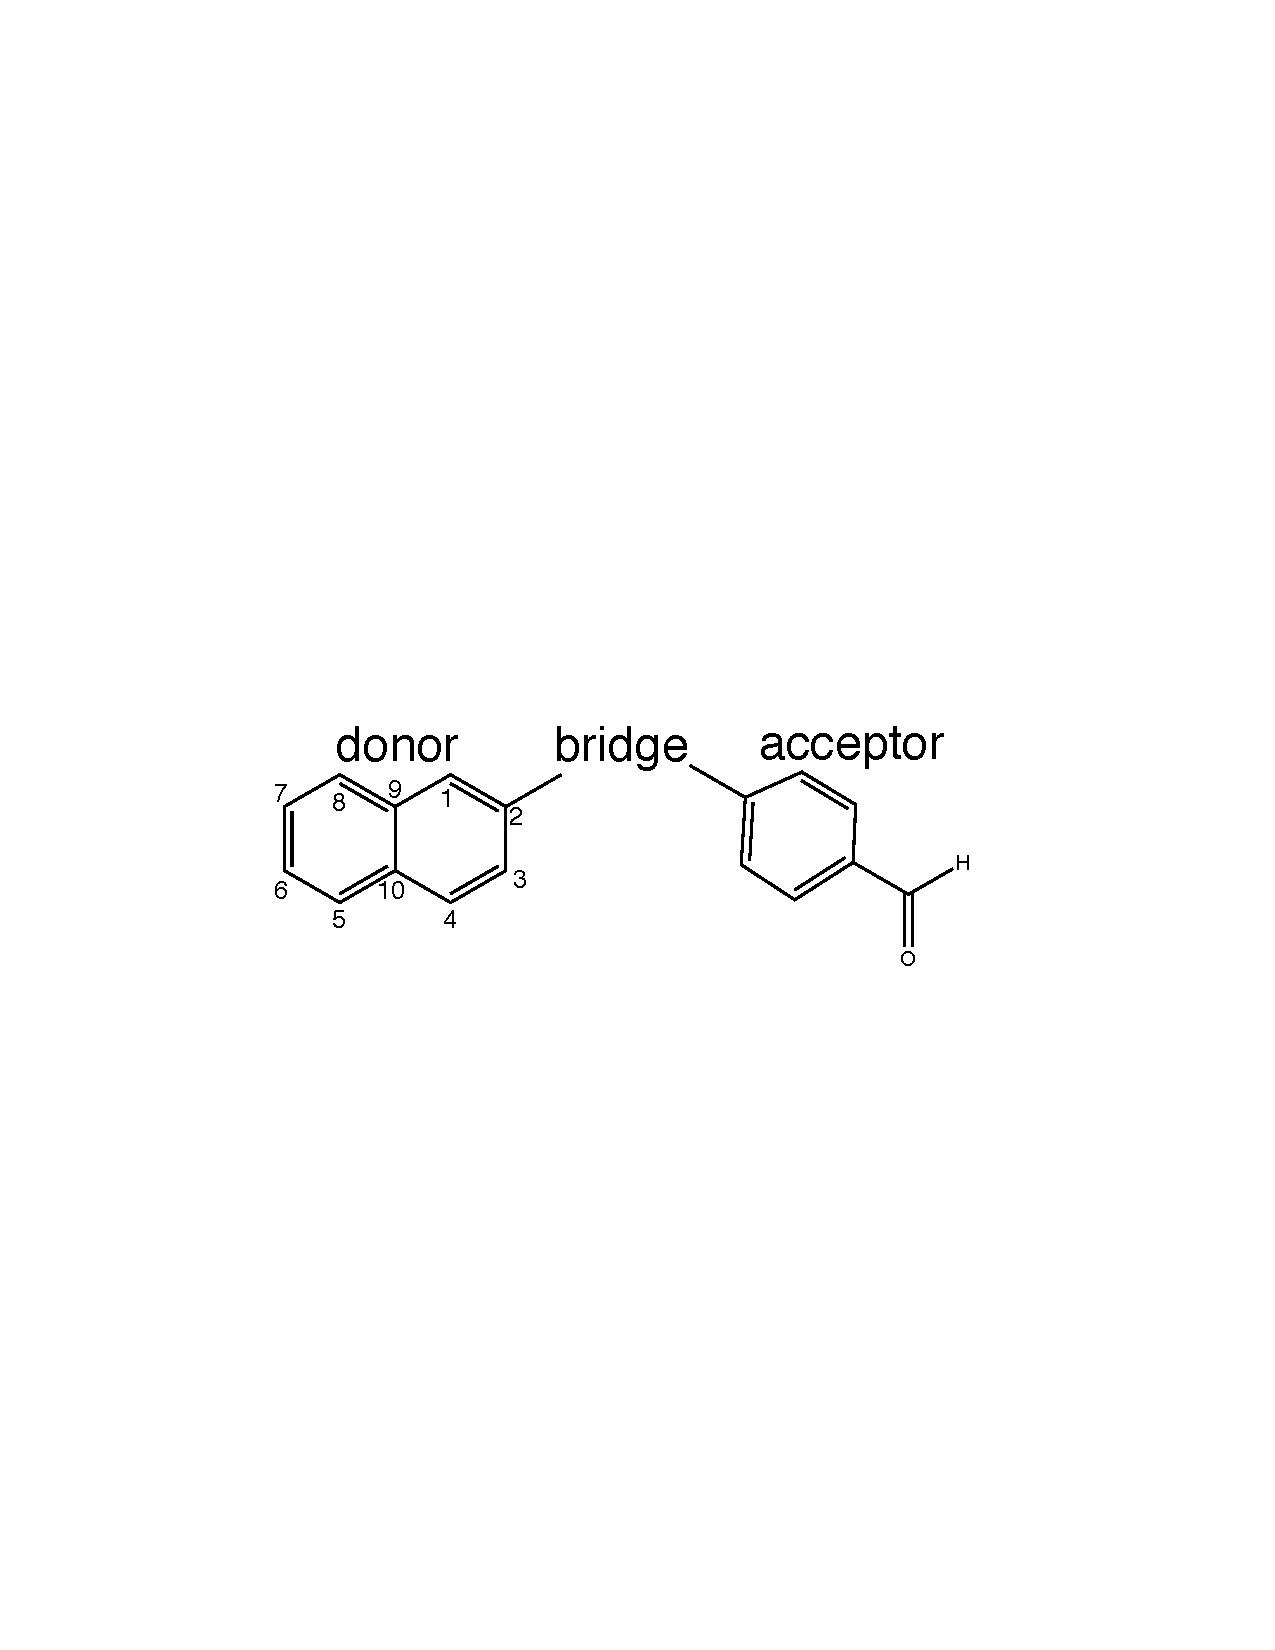
\includegraphics[width=\columnwidth]{Chapters/chap3/molecule1.pdf}
% \caption{Molecular structure of naphthalene donor and a
% benzaldehyde acceptor linked by various bridging units. }\label{struct}
% \end{figure}
% Such systems were the basis of a  classic series of experiments by
% Closs and Miller \cite{miller1984intramolecular,closs1988determination,closs1989connection}
% which verified the existence of the Marcus inverted regime.
% In Ref. \cite{yang2014intramolecular} we showed that both
% the autocorrelation function of the electronic coupling operators
% and the total transfer rate constant calculated using TCLME approach with only PLMs provide an
% excellent approximation to the exact correlation functions and rate
% constants computed using all normal modes, as well as to the experimental
% and recent theoretical values for the transfer rates \cite{subotnik2010predicting}.

In this chapter we analyze the symmetry of PLMs (see Fig. \ref{LanczosModes_chap2}) in model donor-bridge-acceptor systems as projected onto the local
 vibrational modes of the  donor (benzaldehyde)    and  acceptor (naphthalene) moieties.    By constructing the local modes
from the dominant normal modes in the projection,  one can deduce a relation between the PLMs,
fragment modes,  and normal modes for the entire molecule.
% The structure of this paper is as follows. We begin by reviewing the TCLME approach and how one generates the PLMs.
% Below we discuss the symmetry  of PLMs and their relation to a linear coordinate linking the initial/donor geometry to the final/acceptor geometry of the molecule.
%---NEED CONCLUDING STATEMENT----

% \section{Theoretical Model}

% \subsection{Construction and parameterization}
% Our method was detailed in ~Ref. \cite{yang2014intramolecular} but to be self-contained, we briefly present it here.

% \subsection{Model Hamiltonian and transition rates}
% Our theory is initiated by considering a generic model for electronic transitions in the presence of
% nuclear degrees of freedom. Taking the electronic ground state of the system as a reference
% and assuming that the electronic states are coupled linearly to a common set of
%  modes, we arrive a generic form for the Hamiltonian:
%  \begin{eqnarray}
% H=\left(\begin{array}{cc}
% \epsilon_{1} & 0\\
% 0 & \epsilon_{2}
% \end{array}\right)+\left(\begin{array}{cc}
% {\mathbf g}_{11}&{\mathbf g}_{12} \\
% {\mathbf g}_{21} &{\mathbf g}_{22}
% \end{array}\right)\cdot{\mathbf q} +\frac{{\mathbf p}^{2}}{2}+\frac{1}{2}\mathbf{q}^{T}\cdot\mathbf\Omega\cdot\mathbf{q}.
% \nonumber \\
% % \label{ham1}
% \end{eqnarray}
% Here, the first term contains the electronic energies, $\epsilon_{1}$ and $\epsilon_{2}$ computed at a
% reference geometry--typically that of the donor or acceptor state.   The second term represents the
% linearized coupling between the electronic and nuclear degrees of freedom given in terms of the mass-weighted
% normal coordinates $\mathbf q$.   The diagonal terms
% give the adiabatic displacement forces between the reference geometry and the two states.  If we choose one of the
% states as the reference state, then either $\mathbf g_{11}$ or $\mathbf g_{22}$ will vanish.
% The remaining two terms correspond to the harmonic motions of the nuclear normal modes, given here in mass-weighted normal coordinates.
% In the normal mode basis, $\mathbf \Omega$  is diagonal with elements corresponding to the normal mode frequencies, $\omega_{j}^{2}$.

% We now separate Eq. ~\ref{ham1} into diagonal and
% off-diagonal terms
% \begin{eqnarray}
% \hat  H = \hat H_{o} + \hat V
% \end{eqnarray}
% and perform a polaron transform
% using the unitary transformation~\cite{grover1970exciton,rice1994excitons,pereverzev2006time}.
% \begin{eqnarray}
% U&=&e^{-\sum_{ni}\!\!\frac{g_{nni}}{\hbar\omega_i}|n\rangle \langle
% n|(a^{\dagger}_i-a_i)}
%  \nonumber \\
% &=&
% \sum_{n}|n\rangle \langle n|e^{-\sum_{i}\!\!\frac{g_{nni}}{\hbar\omega_i}(a^{\dagger}_i-a_i)}
% \label{unitary}
% \end{eqnarray}
% under which the transformed Hamiltonian is written in terms of the
% diagonal elements
% \begin{eqnarray} \tilde H_0=U^{-1}H_0U
% =\sum_n\tilde\epsilon_n |n\rangle \langle
% n|+\sum_i\omega_ia^{\dagger}_ia_i,
%  \end{eqnarray}
% with  the renormalized electronic energies,
% \begin{eqnarray}
% \tilde\epsilon_n=\epsilon_n-\sum_{i}\frac{g_{nni}^2}{\hbar\omega_i},
% \end{eqnarray}
% and off-diagonal terms,
% \begin{eqnarray} \hat V_{nm}=\sum_{i}g_{nmi}\left(a^{\dagger}_i+
% a_i-\frac{2g_{nni}}{\hbar\omega_i}\right)e^{\sum_{j}\frac{(g_{nnj}-g_{mmj})}{\hbar\omega_j}(a^{\dagger}_j-a_j)}.
% \label{opm}
% \end{eqnarray}
% In the transformed (or dressed) picture the electronic transition from state
% $|n\rangle$ to $|m\rangle$ is accompanied by the excitations of all the
% normal phonon modes.  Transforming to the interaction representation
% and performing a trace over the phonons gives the spectral density in
% terms of the autocorrelation of the electron/phonon coupling
% operators.
% \begin{eqnarray}
% S_{nm}(\tilde\omega) = \int_{-\infty}^{\infty} dt e^{-i\tilde \omega t}C_{nm}(t),\label{spec-dens}
% \end{eqnarray}
% where
% $$
% %C_{nm}(t) = \int_{-\infty}^{\infty} dt e^{-i\tilde \omega t}\langle \hat V_{nm}(t) \hat V_{mn}(0)\rangle.\label{cor-fun}
% C_{nm}(t) =\langle \hat V_{nm}(t) \hat V_{mn}(0)\rangle,\label{cor-fun}
% $$
% is the autocorrelation function of the
% polaron-transformed electron-phonon coupling operator in the Heisenberg representation and
% $\langle \cdots \rangle$ denotes a thermal average over the
% vibrational degrees of freedom.
% The derivation and explicit form for the kernel in Eq.~\ref{spec-dens}  is quite lengthy and is given in
% Ref.~\citenum{pereverzev2006time}.
% Using this approach , the golden-rule rates are given by
% \begin{eqnarray}
% k_{nm}=\lim_{\tau \to \infty}2{\rm Re}\int_{0}^{\tau}dt\left\langle \hat V_{nm}(0)\hat V_{mn}\left(t\right)\right\rangle e^{-i\tilde\omega_{nm}t}.
% \label{gr-expression}
% \end{eqnarray}
% In a practical sense, we take $\tau$ to be some finite time at which the
% autocorrelation function $C(t)$
% has relaxed to zero.

% Later, we will use the $C_{nm}(t) $ to benchmark the convergence of our model with respect to
% the number of nuclear modes included in constructing the electronic coupling operator, $V_{nm}(t)$.
% For our purposes here,  an ``exact''  calculation involves including all nuclear vibrational modes.
% In our previous work we showed that both $C(t)$
% and the total transfer rate constant, $k_{nm}$ calculated using only the first few projected modes provide an
% excellent agreement with the exact quantities computed using  the full set of
% normal modes, as well as the experimental rates,
% when parameterized using accurate quantum chemical data.\cite{yang2014intramolecular}

% \subsection{Hamiltonian and Parameterization}

% We start with the  generic form for the diabatic Hamiltonian, describing two electronic states coupled with $N$ normal modes:
% \begin{eqnarray}
% H_{dia}=\left(\begin{array}{cc}
% \epsilon_{1} & V_{12}\\
% V_{21} & \epsilon_{2}
% \end{array}\right)
% +\left(\begin{array}{cc}
% {\mathbf g}_{11}&{\mathbf g}_{12} \\
% {\mathbf g}_{21} &{\mathbf g}_{22}
% \end{array}\right)\cdot{\mathbf q} +\frac{{\mathbf p}^{2}}{2}+\frac{1}{2}\mathbf{q}^{T}\cdot\mathbf\Omega\cdot\mathbf{q}.
% \nonumber \\
% \end{eqnarray}
% Here, the first term contains the electronic energies, $\epsilon_{1}$ and $\epsilon_{2}$ computed at a
% reference geometry--typically that of the donor or acceptor state. $V_{ij}$ is the diabatic coupling between them.  The second term represents the
% linear coupling between the electronic and nuclear degrees of freedom given in terms of the mass-weighted
% normal coordinates $\mathbf q$.   The diagonal terms
% give the diabatic displacement forces between the reference geometry and the two states.
% The remaining two terms correspond to the harmonic motions of the nuclear normal modes, given here in mass-weighted normal coordinates.
% In the normal mode basis, $\mathbf \Omega$  is diagonal with elements corresponding to the normal mode frequencies, $\omega_{j}^{2}$.

% If we choose one of the states as the reference state, then either $\mathbf g_{11}$ or $\mathbf g_{22}$ will vanish. We further assume Condon approximation to neglect $\mathbf g_{12}$ and $\mathbf g_{21}$. Now the Hamiltonian is simplified to
% \begin{eqnarray}
% H_{dia}=\left(\begin{array}{cc}
% \epsilon_{1} & V_{12}\\
% V_{21} & \epsilon_{2}
% \end{array}\right)+\left(\begin{array}{cc}
% 0 & 0\\
% 0 & 1
% \end{array}\right) {\mathbf g}_{22}\cdot{\mathbf q}+H_{osc},
% \end{eqnarray}
% \label{eq:diaHam}
% where $H_{osc}$ is the harmonic oscillator Hamiltonian for the vibrational normal modes.


% To calculate transition rate, we transform to adiabatic representation. It is done via Edmiston-Ruendenberg (ER) localization \cite{subotnik2010predicting} implemented in Q-Chem and the electronic Hamiltonians
% on adiabatic and diabatic basis are related by the mixing angle $\theta$.
% \begin{equation}
% H_{dia,e}=\left(\begin{array}{cc}
% \cos\theta & -\sin\theta\\
% \sin\theta & \cos\theta
% \end{array}\right)\left(\begin{array}{cc}
% \epsilon_{1}  & 0 \\
% 0  & \epsilon_{2}
% \end{array}\right)\left(\begin{array}{cc}
% \cos\theta & \sin\theta\\
% -\sin\theta & \cos\theta
% \end{array}\right).
% \end{equation}
% The diabatic coupling is then given by
% \begin{eqnarray}
% V_{12}=\frac{1}{2}\sin2\theta\left(\epsilon_{2}-\epsilon_{1}\right).
% \end{eqnarray}
% The full adiabatic Hamiltonian reads:
% \begin{eqnarray}
% H&=&U^{T}H_{dia}U\nonumber  \\
% &=&\left(\begin{array}{cc}
% E_{1}  & 0 \\
% 0 & E_{2}
% \end{array}\right)+\left(\begin{array}{cc}
% \sin^{2}\theta & \frac{1}{2}\sin2\theta\\
% \frac{1}{2}\sin2\theta & \cos^{2}\theta
% \end{array}\right) {\mathbf g}_{22}.{\mathbf q} \nonumber \\
% &+& H_{osc}.\label{eq:locaiHam2}
% \end{eqnarray}
% where the electronic part is in the adiabatic basis with eigenenergies of $E_1$ and $E_2$ at certain reference geometry. The nuclear normal modes are described by $H_{osc}$ whereas $\theta$ is the mixing angle between two states.
% %to describe the coupling between two electronic states, $|1\rangle$ and $|2\rangle$  by a set of nuclear vibrational motionsdescribed by $H_{osc}$.  The angle $\theta$ gives the mixing angle between diabatic states and $E_1$ and $E_{2}$ are electronic energies computed at the same reference configuration.

% To parametrize our Hamiltonian, we assume the diabatic
% are a good approximation to the actual adiabatic potentials.
% This allows us to
% use the gradients of the adiabatic potentials to approximate the diabatic potentials.
% This approximation is  valid when the adiabatic (and diabatic) energy minima
% are far enough away from the crossing points and the mixing angles between the diabatic  and adiabatic
% states is small.
% Thus, all parameters in Eq.~\ref{eq:locaiHam2}  can be  obtained from
% standard  quantum chemical computations.
% As in our previous work, we use the Q-Chem 4.0 package  to obtain the vertical energies
%  from single point CI(S) calculations with 6-31G** basis set at a given
% reference geometry.   We then project the energy gradients onto the vibrational normal
% coordinates

% Our group has shown that the dynamics of Hamiltonian in the form of Eq.~\ref{eq:locaiHam2} can be expressed in a time-convolutionless mater equation \cite{pereverzev2006time}. The derivation is lengthy so we present it briefly.

% \subsection{Transition Rate and Autocorrelation}
% We start from a more general Hamiltonian:
% \begin{eqnarray}
% H=\left(\begin{array}{cc}
% \epsilon_{1} & 0\\
% 0 & \epsilon_{2}
% \end{array}\right)+\left(\begin{array}{cc}
% {\mathbf g}_{11}&{\mathbf g}_{12} \\
% {\mathbf g}_{21} &{\mathbf g}_{22}
% \end{array}\right)\cdot{\mathbf q} +\frac{{\mathbf p}^{2}}{2}+\frac{1}{2}\mathbf{q}^{T}\cdot\mathbf\Omega\cdot\mathbf{q}
% \nonumber \\
% % \label{ham1}
% \end{eqnarray}
% then perform a polaron transform
% using the unitary transformation \cite{grover1970exciton,rice1994excitons,pereverzev2006time}.
% \begin{eqnarray}
% U&=&e^{-\sum_{ni}\!\!\frac{g_{nni}}{\hbar\omega_i}|n\rangle \langle
% n|(a^{\dagger}_i-a_i)}
%  \nonumber \\
% &=&
% \sum_{n}|n\rangle \langle n|e^{-\sum_{i}\!\!\frac{g_{nni}}{\hbar\omega_i}(a^{\dagger}_i-a_i)}
% % \label{unitary}
% \end{eqnarray}
% under which the transformed Hamiltonian is written in terms of the
% diagonal elements
% \begin{eqnarray} \tilde H_0=U^{-1}H_0U
% =\sum_n\tilde\epsilon_n |n\rangle \langle
% n|+\sum_i\omega_ia^{\dagger}_ia_i,
%  \end{eqnarray}
% with  the renormalized electronic energies,
% \begin{eqnarray}
% \tilde\epsilon_n=\epsilon_n-\sum_{i}\frac{g_{nni}^2}{\hbar\omega_i},
% \end{eqnarray}
% and off-diagonal terms,
% \begin{eqnarray} \hat V_{nm}=\sum_{i}g_{nmi}\left(a^{\dagger}_i+
% a_i-\frac{2g_{nni}}{\hbar\omega_i}\right)e^{\sum_{j}\frac{(g_{nnj}-g_{mmj})}{\hbar\omega_j}(a^{\dagger}_j-a_j)}.
% % \label{opm}
% \end{eqnarray}
% % In the transformed (or dressed) picture the electronic transition from state
% % $|n\rangle$ to $|m\rangle$ is accompanied by the excitations of all the
% % normal phonon modes.  Transforming to the interaction representation
% % and performing a trace over the phonons gives the spectral density in
% % terms of the autocorrelation of the electron/phonon coupling
% % operators.
% % \begin{eqnarray}
% % S_{nm}(\tilde\omega) = \int_{-\infty}^{\infty} dt e^{-i\tilde \omega t}C_{nm}(t),\label{spec-dens}
% % \end{eqnarray}
% % where
% % $$
% %C_{nm}(t) = \int_{-\infty}^{\infty} dt e^{-i\tilde \omega t}\langle \hat V_{nm}(t) \hat V_{mn}(0)\rangle.\label{cor-fun}
% After lengthy derivation we get the autocorrelation function in the Heisenberg representation
% $$
% C_{nm}(t) =\langle \hat V_{nm}(t) \hat V_{mn}(0)\rangle,\label{cor-fun}
% $$
% where $\langle \cdots \rangle$ denotes a thermal average over the
% vibrational degrees of freedom.
% % The derivation and explicit form for the kernel in Eq.~\ref{spec-dens}  is quite lengthy and is given in
% % Ref.~\citenum{pereverzev2006time}.
% Using this approach , the golden-rule rates are given by
% \begin{eqnarray}
% k_{nm}=\lim_{\tau \to \infty}2{\rm Re}\int_{0}^{\tau}dt\left\langle \hat V_{nm}(0)\hat V_{mn}\left(t\right)\right\rangle e^{-i\tilde\omega_{nm}t}.
% % \label{gr-expression}
% \end{eqnarray}
% In a practical sense, we take $\tau$ to be some finite time at which the
% autocorrelation function $C(t)$
% has relaxed to zero.

% Later, we will use the $C_{nm}(t) $ to benchmark the convergence of our model with respect to
% the number of nuclear modes included in constructing the electronic coupling operator, $V_{nm}(t)$.
% For our purposes here,  an ``exact''  calculation involves including all nuclear vibrational modes.
% In our previous work we showed that both $C(t)$
% and the total transfer rate constant, $k_{nm}$ calculated using only the first few projected modes provide an
% excellent agreement with the exact quantities computed using  the full set of
% normal modes, as well as the experimental rates,
% when parameterized using accurate quantum chemical data \cite{yang2014intramolecular}.


% % Diagonalizing $H$ at a given nuclear configuration  provides the adiabatic potentials for our system, which can be used to approximate the diabatic potentials.

% % The linear coupling parameter $ {\mathbf g}_{22}$ defines
% % a force
% % along a vector connecting the
% % the initial and final equilibrium geometries of the molecule.
% % This vector, along with the diabatic mixing angle can be obtained from quantum chemistry
% % using the ER localization
% % scheme to approximate the donor and acceptor states.
% % By analyzing this force we can gain the insight into the dynamics of the transition as well as
% % open an avenue for developing improved approximations for transition rates.
% % In our previous work \cite{yang2014intramolecular},  we presented a Lanczos-base ranking algorithm that project
% % out a series of nuclear displacements that are most important for
% % the transition.   We refer to the highest-ranked mode identified by the algorithm
% % as the ``primary Lanczos mode'' (PLM).


% % \subsection{Computing spectral densities and transition rates}

% % Once a suitable set of parameters and vibrational modes  have been determined,





% \subsection{Constructing Primary Lanczos Modes}
% The linear coupling parameter $ {\mathbf g}_{22}$ in Eq.~\ref{eq:locaiHam2} defines
% a force
% along a vector connecting
% the initial and final equilibrium geometries of the molecule.
% This vector, along with the diabatic mixing angle can be obtained from quantum chemistry
% using the ER localization
% scheme to approximate the donor and acceptor states.
% By analyzing this force we can gain the insight into the dynamics of the transition as well as
% open an avenue for developing improved approximations for transition rates.
% In our previous work \cite{yang2014intramolecular},  we presented a Lanczos-base ranking algorithm that project
% out a series of nuclear displacements that are most important for
% the transition.   We refer to the highest-ranked mode identified by the algorithm
% as the ``primary Lanczos mode'' (PLM).
% The process of finding the PLMs is initiated by defining the vector ${\mathbf v}_{1} = {\mathbf g}_{22}$.
% At each step indexed by $k$,  we define a projection operator
% \begin{eqnarray}
% {\mathbf P}_{k} = {\mathbf v}_{k}\otimes  {\mathbf v}_{k}
% \end{eqnarray}
% and its complement ${\mathbf Q}_{k} = {\mathbf I}  - {\mathbf P}_{k}$.
% We also construct
% \begin{eqnarray}
% \mathbf p = \sum_{k} \mathbf P_{k}
% \end{eqnarray}
% as  the total projection operator for all ${k} \le N$ modes.
% We then project the Hessian matrix $\mathbf\Omega$ into each subspace {\em viz.}
% \begin{eqnarray}
% \mathbf\Omega_{p} = \mathbf P_{k}\cdot \mathbf\Omega \cdot \mathbf P_{k} \,\, \& \,\, \mathbf\Omega_{q} = \mathbf Q_{k}\cdot \mathbf\Omega \cdot  \mathbf Q_{k}
% \end{eqnarray}
% and diagonalize each to obtain eigenvalues and eigenvectors $\{\alpha_{p}, {\mathbf M}_{p}\}$ and $\{\alpha_{q}, {\mathbf M}_{q}\}$
% respectively.  $\mathbf\Omega_{p} $ and $\mathbf\Omega_{q}$ are $N\times N$ matrices.
% The first set of these  will have a single
% non-trivial eigenvalue and the second set
% will have $N-k$ non-trivial eigenvalues. We then collect the non-trivial eigenvectors associated with each
% to form the orthogonal transformation matrix
% \begin{eqnarray}
% {\mathbf M}_{k} = \{{\mathbf M}_{p},{\mathbf M}_{q}\}.
% \end{eqnarray}
% and again transform the full Hessian $\mathbf\Omega$ into this new vector space to form the $N\times N$ matrix $\mathbf\Omega'$.
%  At each step in the iteration, the transformed Hessian, $\mathbf\Omega'$ is in the form of a
% $k\times k$ tri-diagonal submatrix in the upper-left part of the matrix and
% a diagonal submatrix in the lower-right.


% \begin{figure*}[t]
% \subfloat[c-1,4ee]{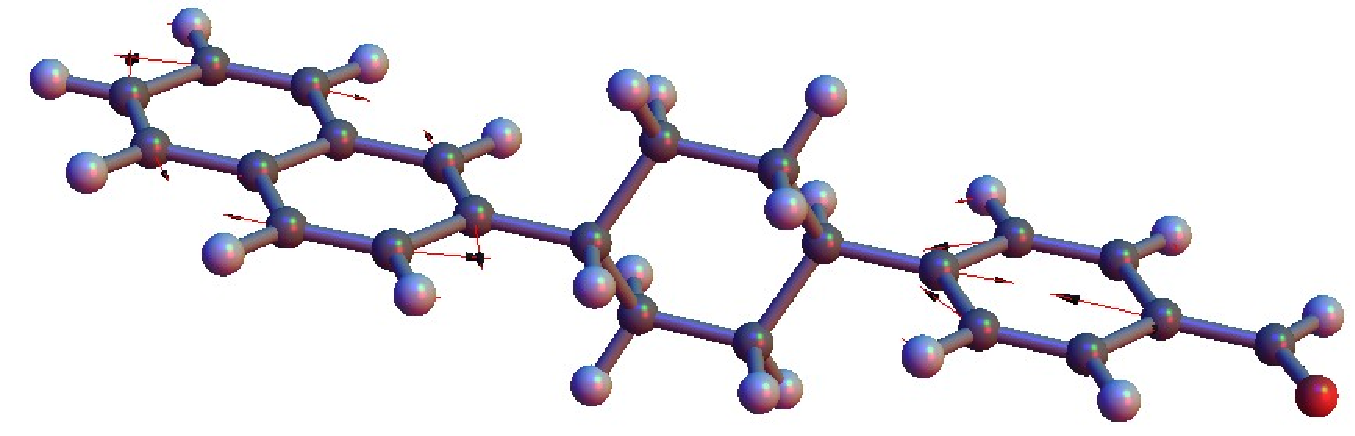
\includegraphics[width=0.75\columnwidth]{Chapters/chap3/Figure1a.pdf}}\\
% \subfloat[d-2,6ae]{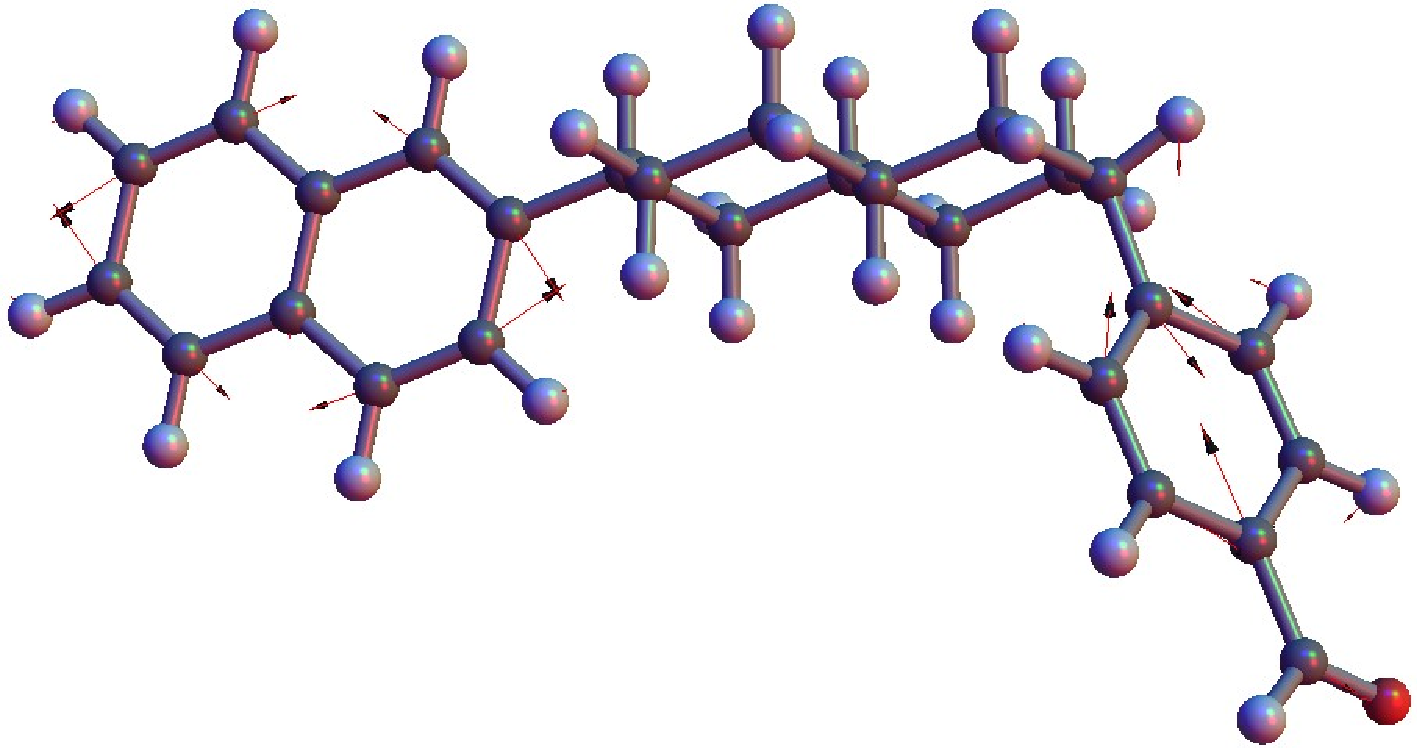
\includegraphics[width=0.75\columnwidth]{Chapters/chap3/Figure1b.pdf}}
% \caption{
% Primary Lanczos modes for (a) c-1,4ee and (b) d-2,6ae projected onto the atomic displacement coordinates.  The frequencies
% for both these are at 0.185 eV (1490 cm$^{-1}$), a typical $C=C$ stretching frequency for arene systems.
% }\label{LanczosModes}
% \end{figure*}


% In Fig.~\ref{LanczosModes_chap2}  we show the PLMs for the
% intramolecular triplet energy transfer within
% two representative donor-bridge-acceptor molecules from our study, termed c-1,4ee and d-2,6ae.
% In both cases, triplet energy is transferred from a benzaldehyde (BZ) donor group to a naphthyl- acceptor group.
% Several observations can be made from Fig.~\ref{LanczosModes_chap2} concerning the primary Lanczos modes for these
% donor-bridge-acceptor systems. First, there is negligible contribution from the bridging unit.
% This is not surprising since the transitions involve  electronic energy
%  transfer between $\pi$-orbitals localized on the donor and acceptor moieties.
%  Since the bridges in these cases
% are not conjugated, there is very weak electronic coupling between the D/A groups and the bridge itself.
% Hence, to a good approximation, the electronic
% contribution from the bridge can be effectively ignored, it simply serves to hold the donor and acceptor in fixed relative positions.
% Secondly, the displacement vectors on donor and acceptor moieties are very much akin to  totally symmetric normal modes
% of the corresponding moieties, and do not correspond any single normal vibrational  mode of the whole molecule.

In the next two sections, we discuss the symmetry  of PLMs and their relation to a linear coordinate linking the initial/donor geometry to the final/acceptor geometry of the molecule. We first project the PLMs onto the normal modes of both the donor or acceptor moieties
and onto entire molecules (donor-bridge-acceptor).  Using these reduced PLMs we
 compute rate constants and compare to the numerically exact results obtained using the full
modes.  Then we do a similar set of projections using simply the geometric change from initial to final configurations
to explore  the relation between the PLMs and geometry.



\section{Symmetry of the Primary Lanczos Modes}

Fig.~\ref{fragProj} shows the projection of the PLMs  onto the normal modes of
donor and acceptor moieties in molecules of c-1,4ee and d-2,6ae, respectively.
In each case, we label the dominant contributions by the
irreducible representations (IR) of the moiety.
There are 4 sets of normal modes used as basis in projections. Two are the normal modes of benzaldehyde and two of naphthalene. They are generated as follows: first, we take the  coordinates of benzaldehyde  and naphthalene from the equilibrium geometry of c-1,4ee and d-2,6ae, and add necessary hydrogens. In theory, naphthalene has $D_{2h}$ symmetry. However, by taking coordinates directly from the D-B-A molecules, the geometry of naphthalene is distorted slightly by the bridge and acceptor moieties, and its point group reduces to $C_{1}$. We want the naphthalene to have high symmetry, so we can use the irreducible representations of $D_{2h}$ to classify its normal modes. As the result, we use GaussView 5 to enforce $D_{2h}$ symmetry on naphthalene. For  benzaldehyde, we leave  the coordinates unchanged, as there is no obvious way to increase the symmetry for benzaldehyde. Finally we run frequency computations for all 4 sets of coordinates.
% The normal mode basis is generated as follows:
% first, we take the geometry of donor or acceptor moiety and add  the necessary hydrogens.
% Then the $D_{2h}$ symmetry is applied to naphthalene using GaussView 5.
% The benzaldehyde moiety is unchanged because it has very low  symmetry:  $C_{s}$ if planar and $C_{1}$  otherwise.

\begin{figure*}[]
\subfloat[]{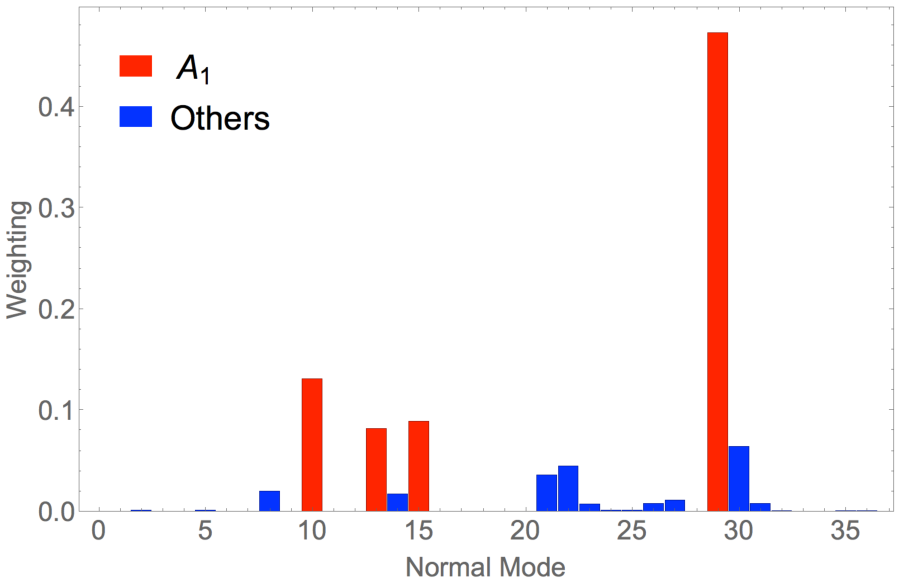
\includegraphics[width=0.49\columnwidth]{Chapters/chap3/Figure2a.pdf}}
\subfloat[]{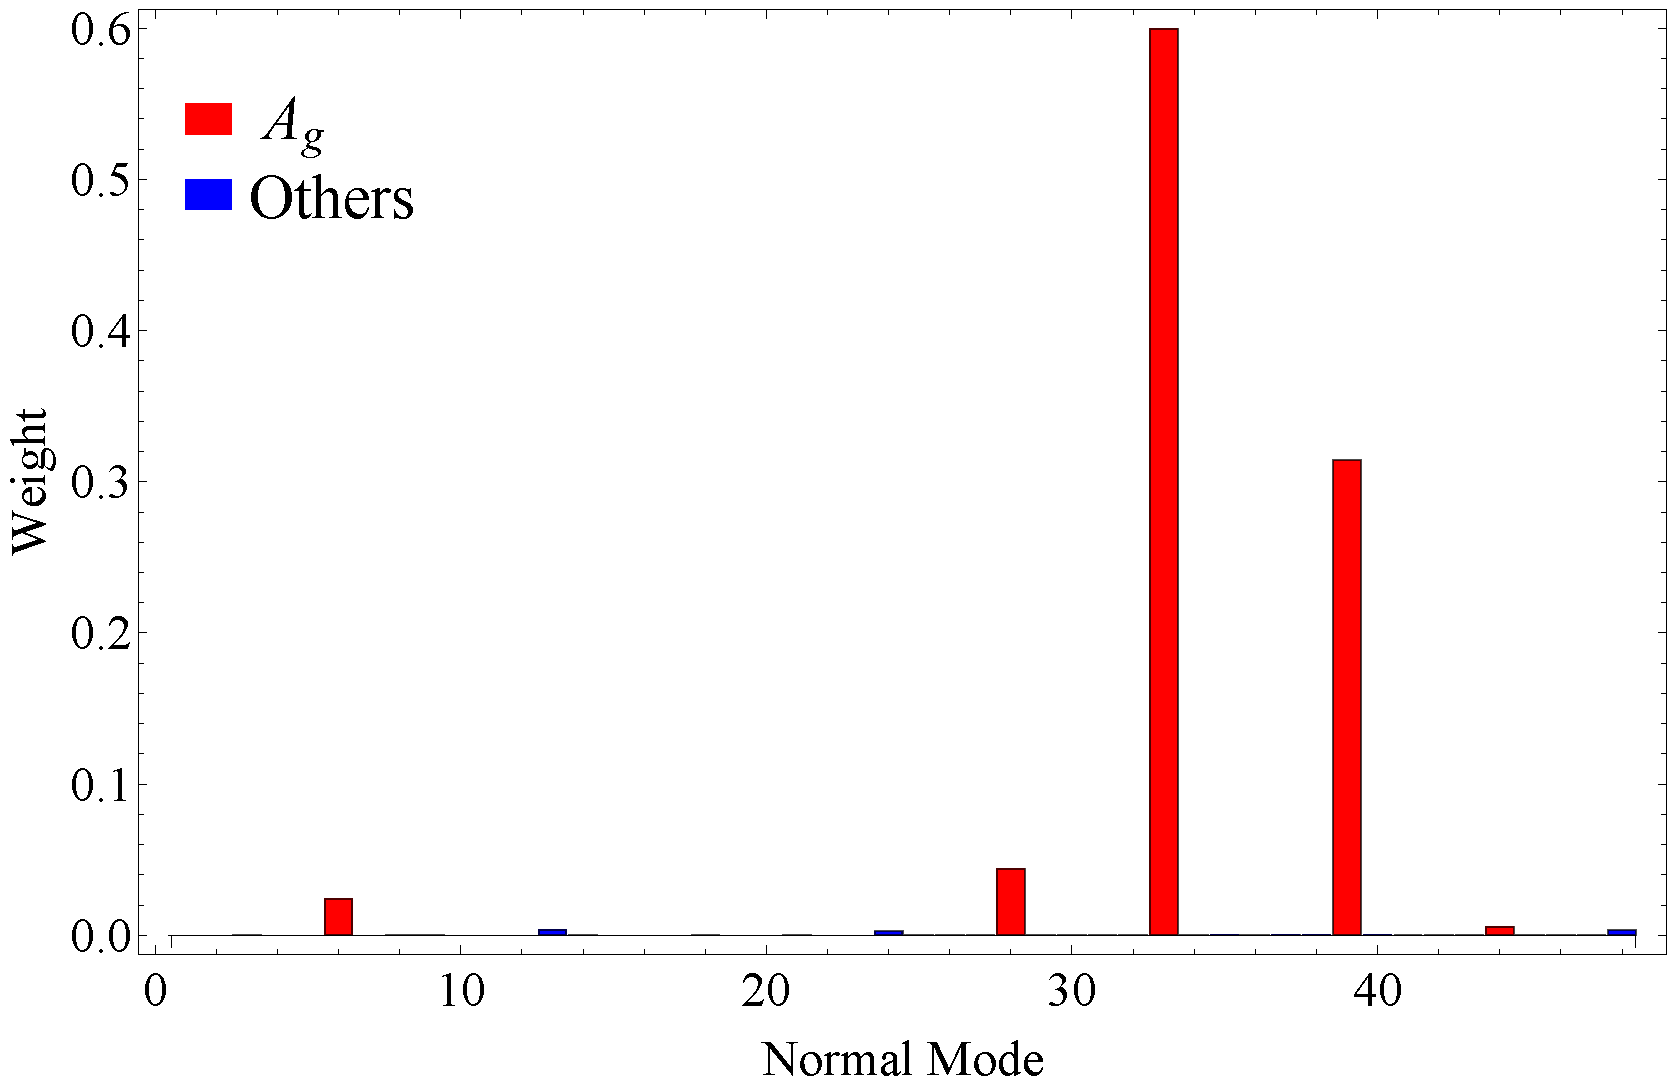
\includegraphics[width=0.49\columnwidth]{Chapters/chap3/Figure2b.pdf}} \\
\subfloat[]{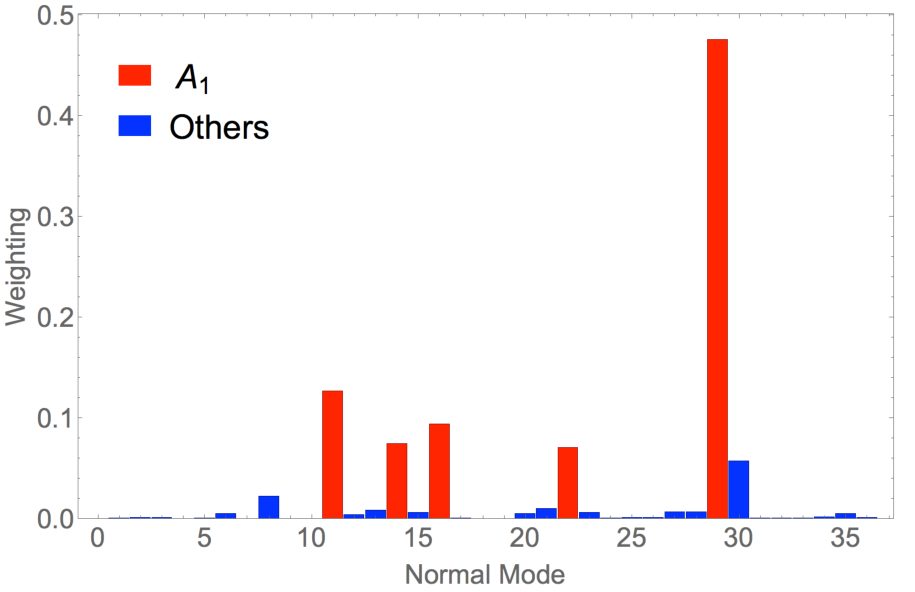
\includegraphics[width=0.49\columnwidth]{Chapters/chap3/Figure2c.pdf}}
\subfloat[]{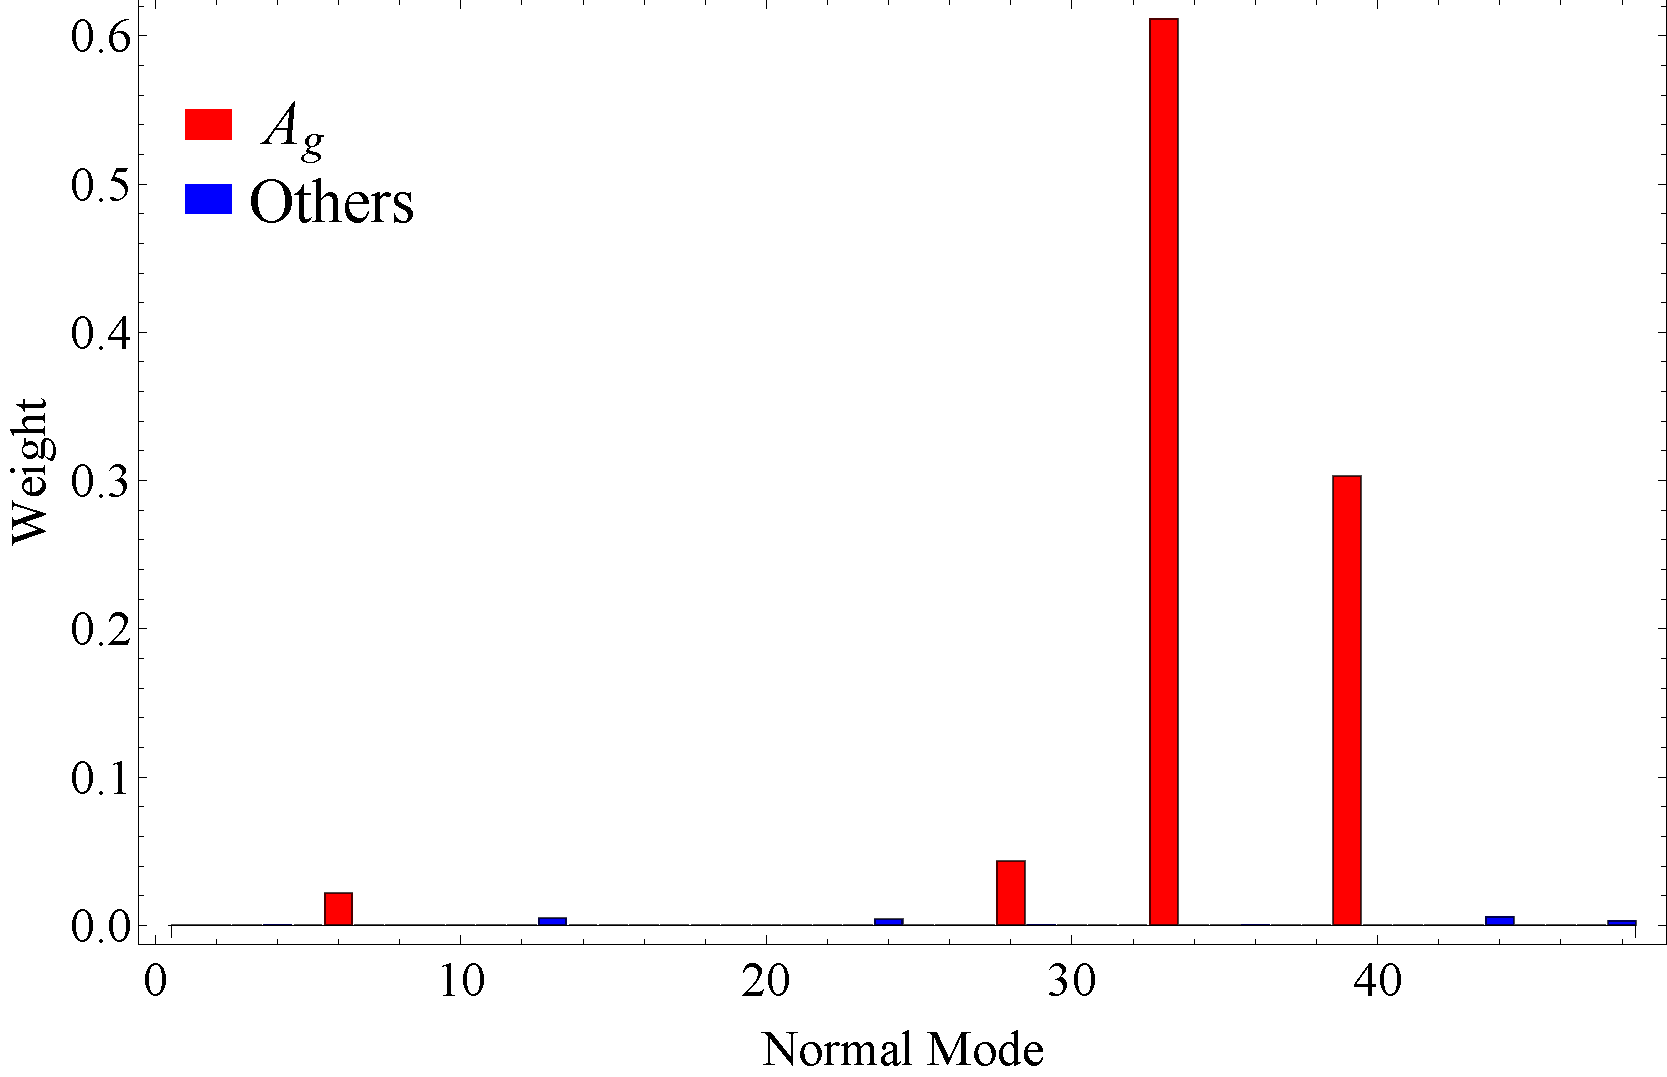
\includegraphics[width=0.49\columnwidth]{Chapters/chap3/Figure2d.pdf}}
\caption{Projection of PLMs onto (a) benzaldehyde in c-1,4ee (b) symmetrized naphthalene in c-1,4ee, (c) benzaldehyde in d-2,6ae and (d) symmetrized naphthalene in d-2,6ae.
The normal modes are listed from low to high frequency and the irreducible representations of the dominant modes are color-coded. The assigned IRs for naphthalene are exact
 whereas the IRs are only approximate for benzaldehyde. \label{fragProj}}
\end{figure*}


If one treats the aldehyde group as a local site, one can classify the ring-motions of
benzaldehyde in terms of the $C_{2v}$ irreducible representations.
As a result, the assigned irreducible representations are exact for naphthalene but approximate for benzaldehyde.
We then assign a weight to each mode viz.
$$
w_i = \frac{\left\langle \overrightarrow{M_{i}}|\overrightarrow{PLM}\right\rangle ^{2}}{\sqrt{\sum_{i}\left\langle \overrightarrow{M_{i}}|\overrightarrow{PLM}\right\rangle ^{2}}}
$$
where $\overrightarrow{M_{i}}$ is the displacement vector of the $i$th normal mode, and $\overrightarrow{PLM}$ is the displacement vector of the PLM on the corresponding moiety. For example, for naphthalene, the $\overrightarrow{PLM}$ are the vectors in Fig. \ref{LanczosModes_chap2}, with only the atoms of naphthalene kept.
The symmetrization of naphthalene introduces a subtle problem. The $\overrightarrow{PLM}$  is based on the distorted geometry of naphthalene in the D-B-A molecule, while $\overrightarrow{M_{i}}$ is computed on the geometry of symmetrized naphthalene. Two geometries differ slightly, so $\left\langle \overrightarrow{M_{i}}|\overrightarrow{PLM}\right\rangle$ depends on how we orient them.
We choose to orient the original and symmetrized frames by first aligning the center of masses
and then minimize the RMS displacement between atoms. This is arbitrary. Fortunately, two geometries are really similar, so we expect the choice of orientation, as long as it is not ridiculous, is acceptable.
By analyzing the projections it becomes clear that in all cases, the dominant components
belong to totally symmetric $A_{g}$ or $A_1$ irreducible representations,  in agreement
with the intuitive observations from Fig.~\ref{LanczosModes_chap2}.

This behavior is not unique for the napthyl-bridge-benzaldehyde  system.
To see this, we repeated the analysis by replacing naphthalene with various acceptor groups, as shown in Fig.~\ref{benz}. Fig.~\ref{benz} also shows the corresponding PLMs and correlation functions.
% and d-2,6ae and compute the
%coupling correlation functions in Eq.~\ref{cor-fun} and displacement vectors of their
%PLMs.  Fig.~\ref{benz} shows the correlation functions and PLMs for  two phenyl-[bridge]-BZ
For both molecules,  4 projected modes are enough to reproduce the exact (all modes) correlation function up to 10 fs. It indicates that
the projection scheme provides an accurate description of the electronic coupling in  these cases as well.
%Moreover, the PLMs in each case are similar to the PLMs in the napthyl-[bridge]-BZ
Moreover, the PLMs in Fig.~\ref{benz} are qualitatively similar to those in Fig.~\ref{LanczosModes_chap2}, where the acceptor is naphthalene.
The displacements vectors on the benzaldehyde moiety in all 4 molecules are almost identical, and  the displacements vectors on the naphthalene, phenyl and anthracene moieties all belong to totally symmetric irreducible representations.

%Till now we have shown that in the donor and acceptor moieties, PLMs are collections of normal modes with totally symmetric representation. I
%
%In next section we'll show that several of these normal modes of donor and acceptor
%are enough to recover the PLM of the whole molecule, namely, the bridge is negligible.


%\begin{figure*}[tbh]
%\subfloat[]{\includegraphics[width=0.95\columnwidth]{Chapters/chap3/C14eeBenzaldehydeProj.pdf}}
%\subfloat[]{\includegraphics[width=0.95\columnwidth]{Chapters/chap3/C14eeNaphSymmProj.pdf}} \\
%\subfloat[]{\includegraphics[width=0.95\columnwidth]{Chapters/chap3/D26aeBenzaldehydeProj.pdf}}
%\subfloat[]{\includegraphics[width=0.95\columnwidth]{Chapters/chap3/D26aeNaphSymmProj.pdf}}
%\caption{Projection of PLMs onto (a) benzaldehyde in c-1,4ee (b) symmetrized naphthalene in c-1,4ee, (c) benzaldehyde in d-2,6ae and (d) symmetrized naphthalene in d-2,6ae.
%The normal modes are listed from low to high frequency and the irreducible representations of the dominant modes are colorcoded. The assigned IRs for naphthalene are exact
% whereas the  IRs are only approximate for benzaldehyde. \label{fragProj}}
%\end{figure*}

\begin{figure*}[]
\subfloat[]{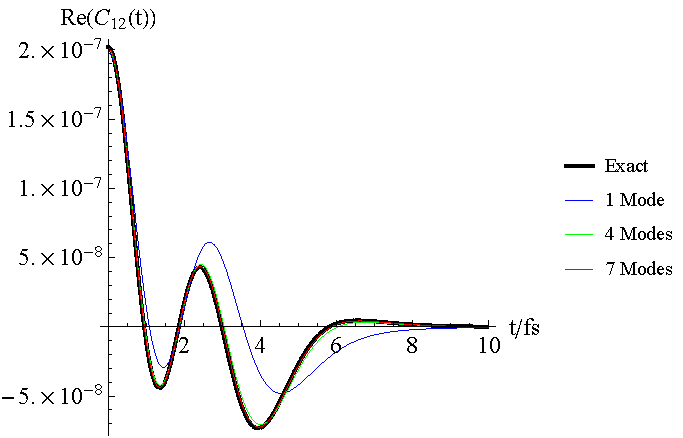
\includegraphics[width=0.49\columnwidth]{Chapters/chap3/Figure3a.pdf}}
\subfloat[]{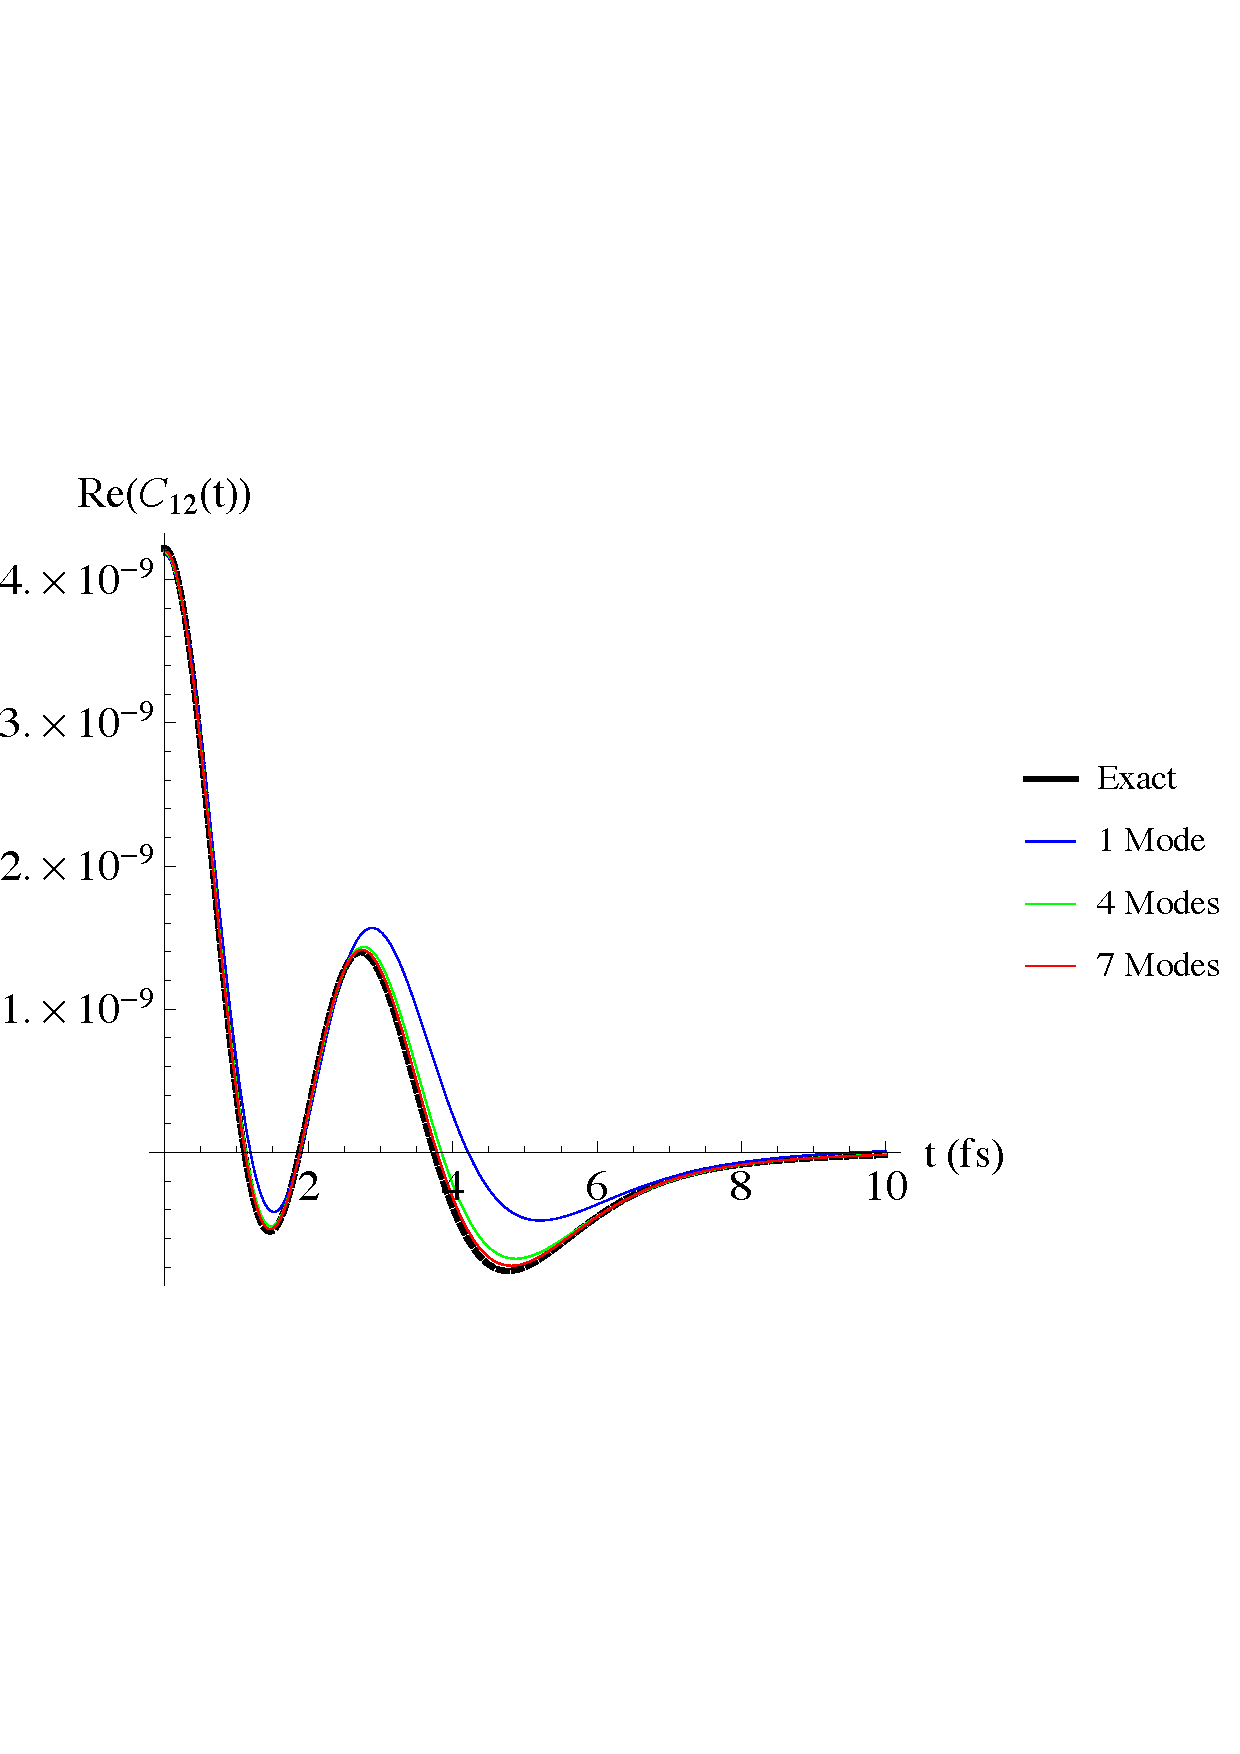
\includegraphics[width=0.49\columnwidth]{Chapters/chap3/Figure3b.pdf}}\\
\subfloat[]{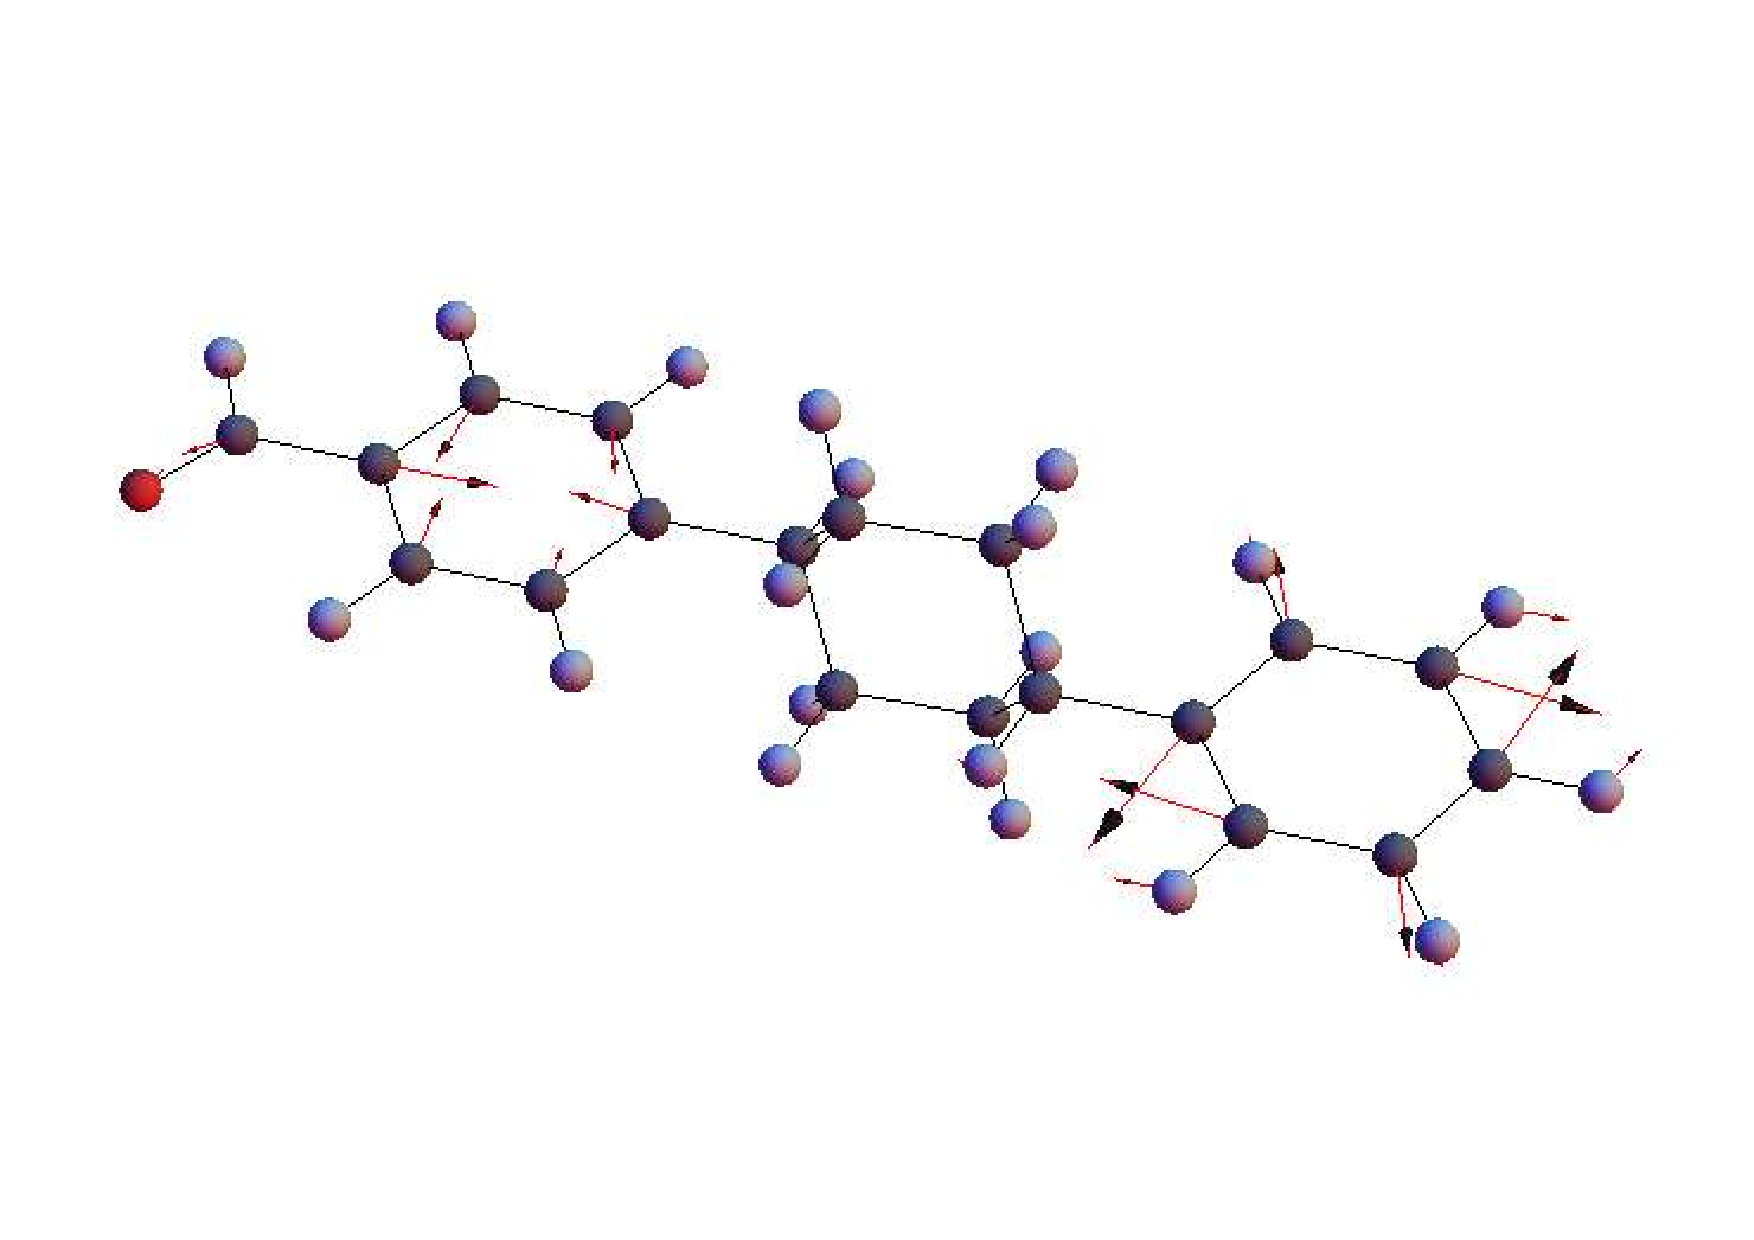
\includegraphics[width=0.49\columnwidth]{Chapters/chap3/Figure3c.pdf}}
\subfloat[]{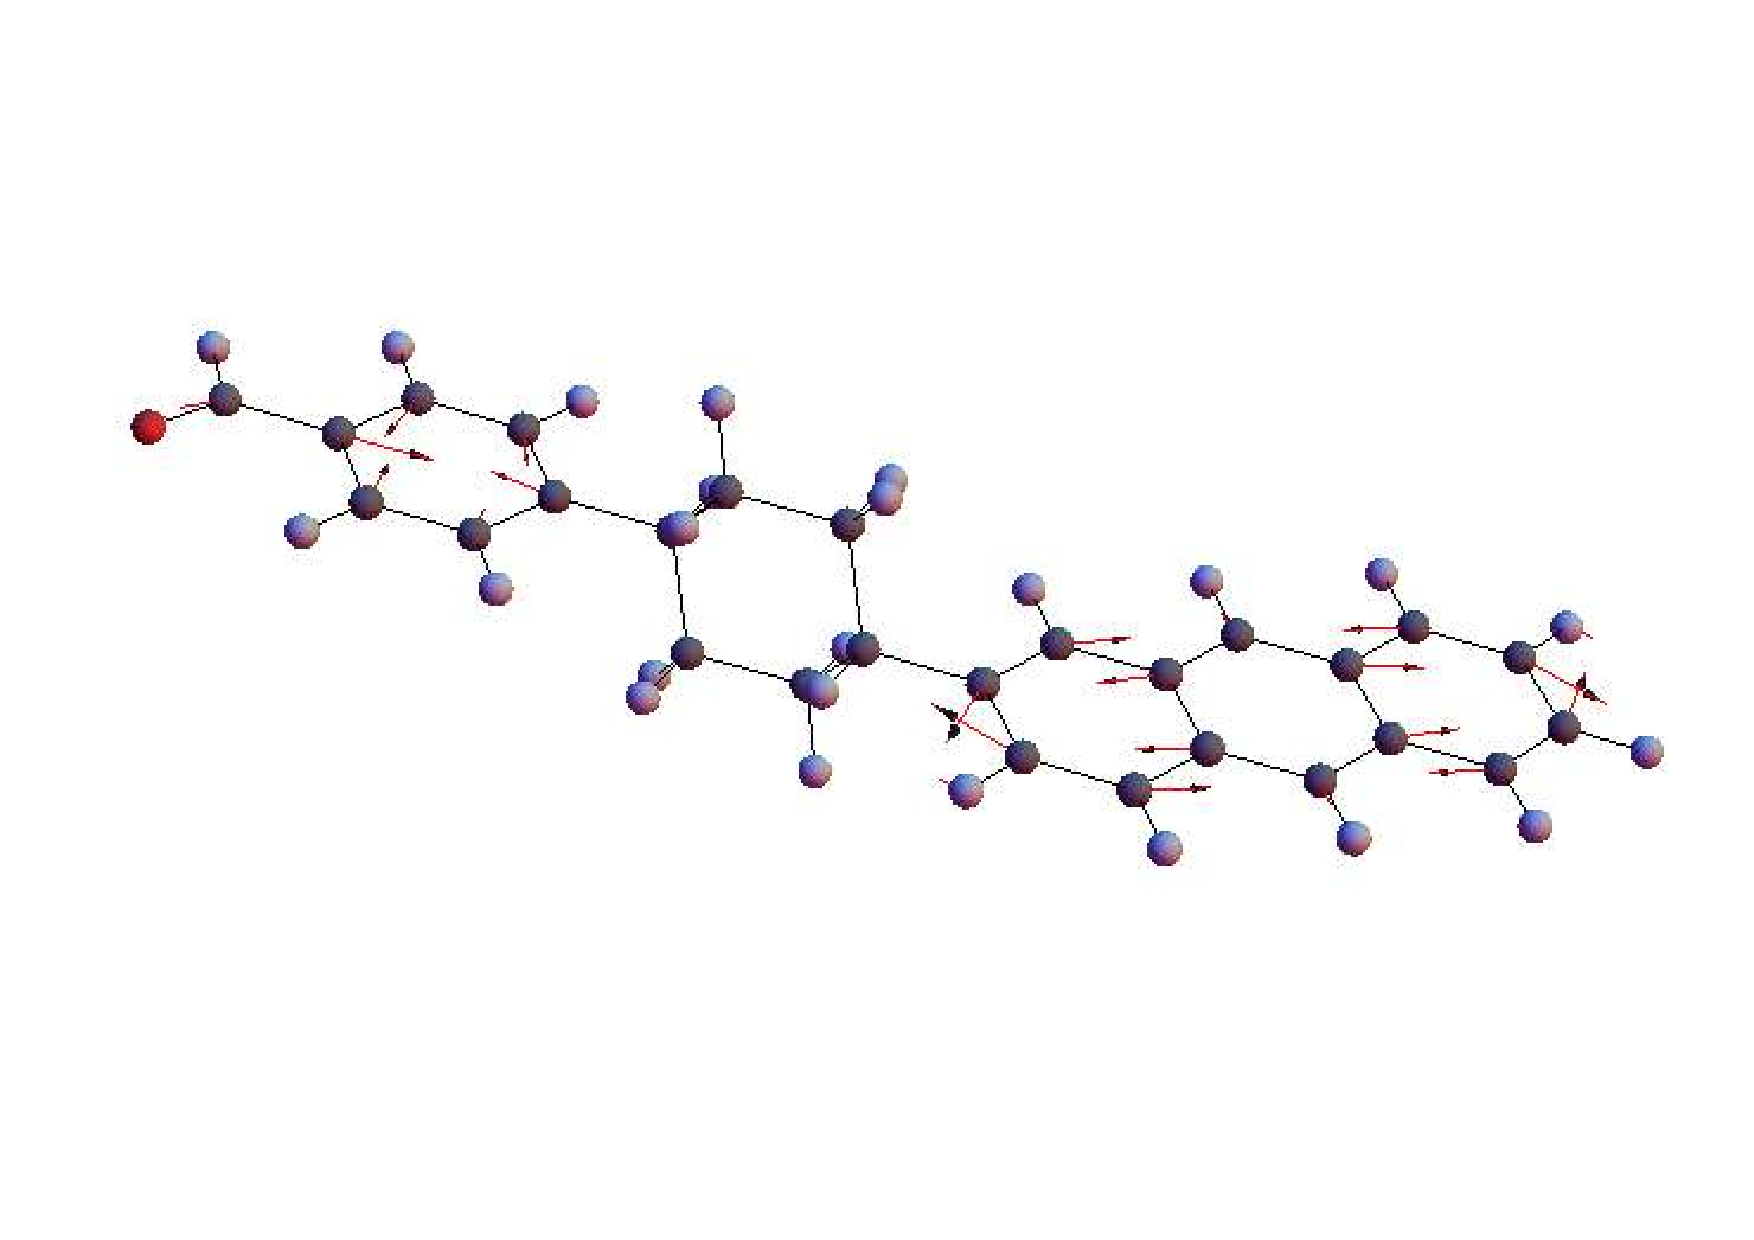
\includegraphics[width=0.49\columnwidth]{Chapters/chap3/Figure3d.pdf}}
%\subfloat[]{\includegraphics[width=0.45\columnwidth]{Chapters/chap3/benzeneC14ee10fs.pdf}}
%\subfloat[]{\includegraphics[width=0.45\columnwidth]{Chapters/chap3/benzeneD26ae10fs.pdf}}
%\subfloat[]{\includegraphics[width=0.45\columnwidth]{Chapters/chap3/PrimeModeBenzeneC14ee.pdf}}
%\subfloat[]{\includegraphics[width=0.45\columnwidth]{Chapters/chap3/PrimeModeBenzeneD26ae.pdf}}
\caption{The correlation functions of projected modes for c-1,4ee with the naphthalene moiety
replaced by (a) phenyl ring and (b) anthracene, with their PLMs shown in (c) and (d). \label{benz}}
%\caption{The correlation function of PLM compared to the exact one calculated with all normal modes for the (a) c-1,4ee (b) d-2,6ae, with naphthalene replaced by phenyl ring.Their PLMs are in (c) for c-1,4ee and (d) for d-2,6ae.\label{benz}}
\end{figure*}

\begin{figure*}[th]
\subfloat[]{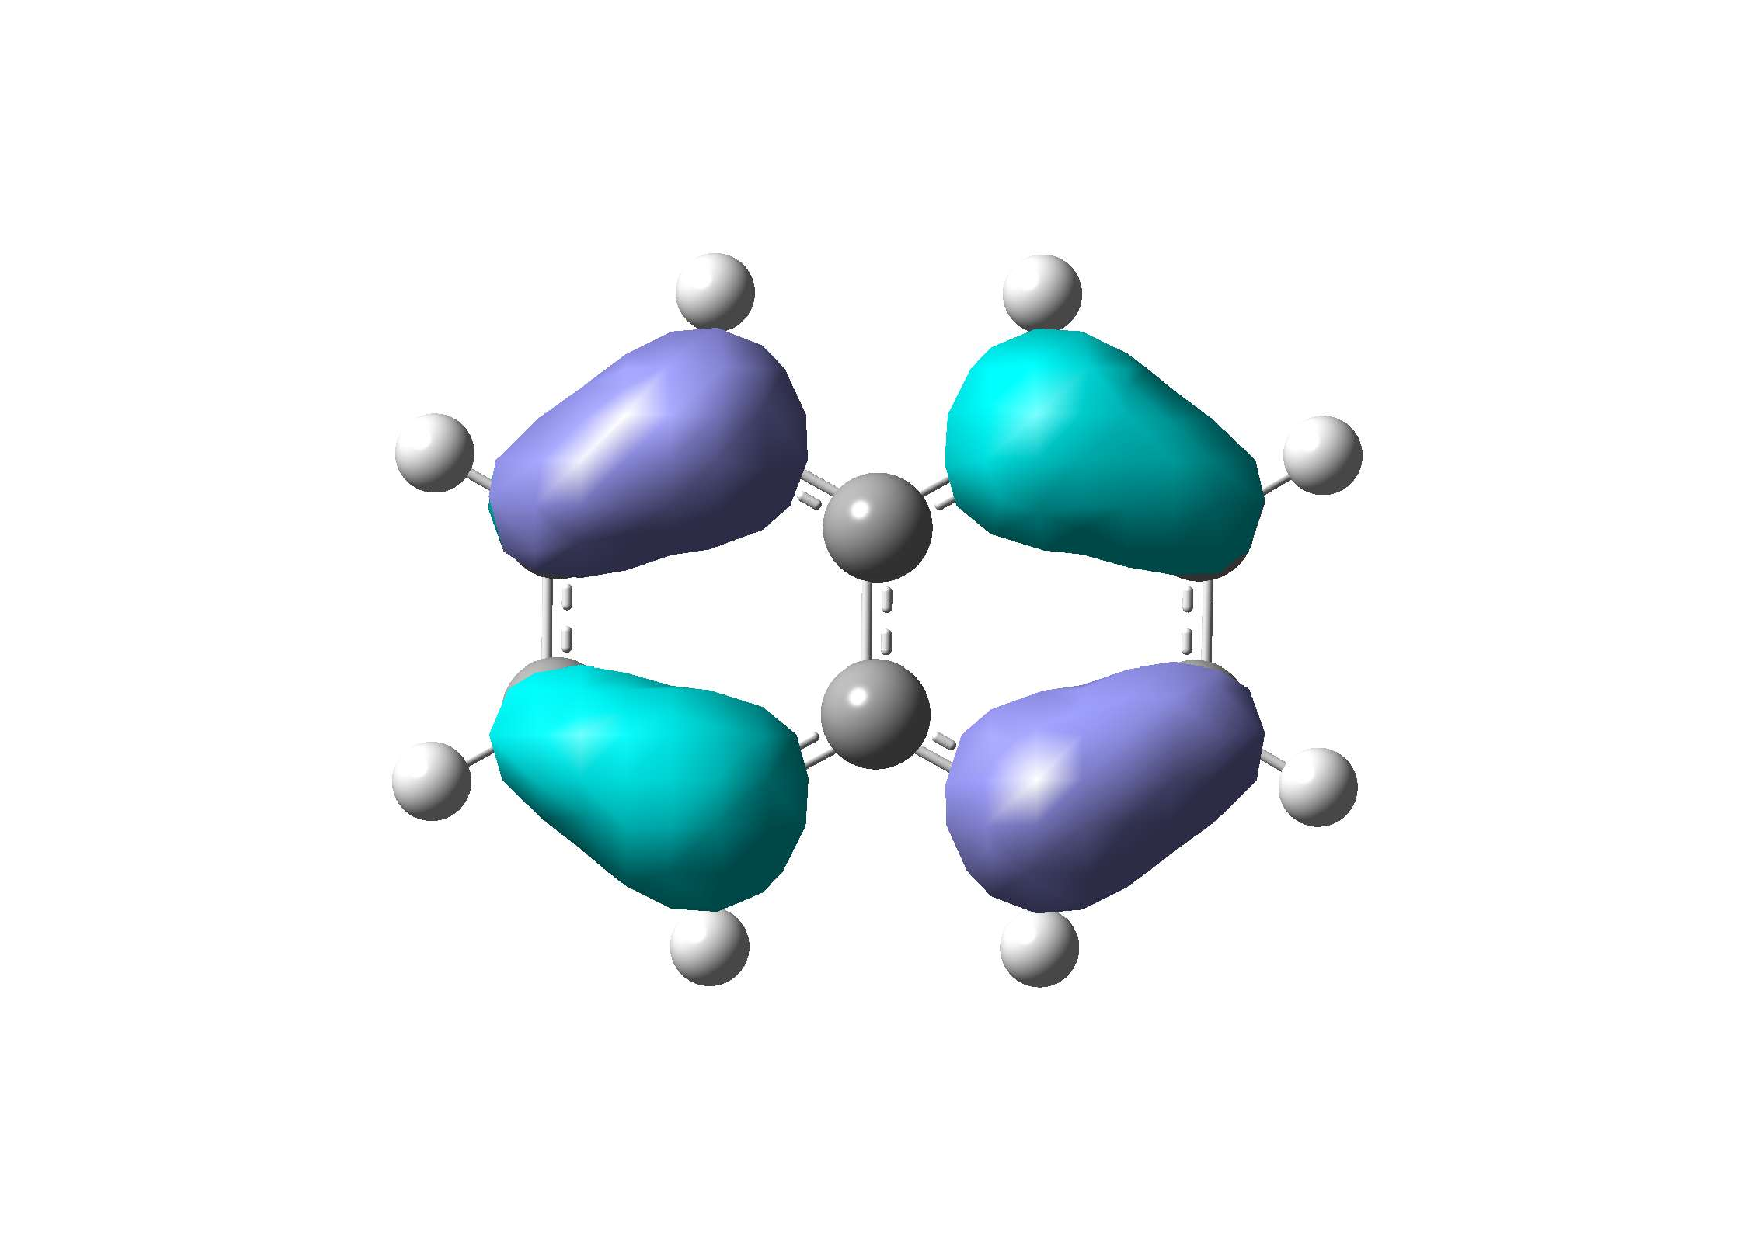
\includegraphics[width=0.45\columnwidth]{Chapters/chap3/Figure4a.pdf}}
\subfloat[]{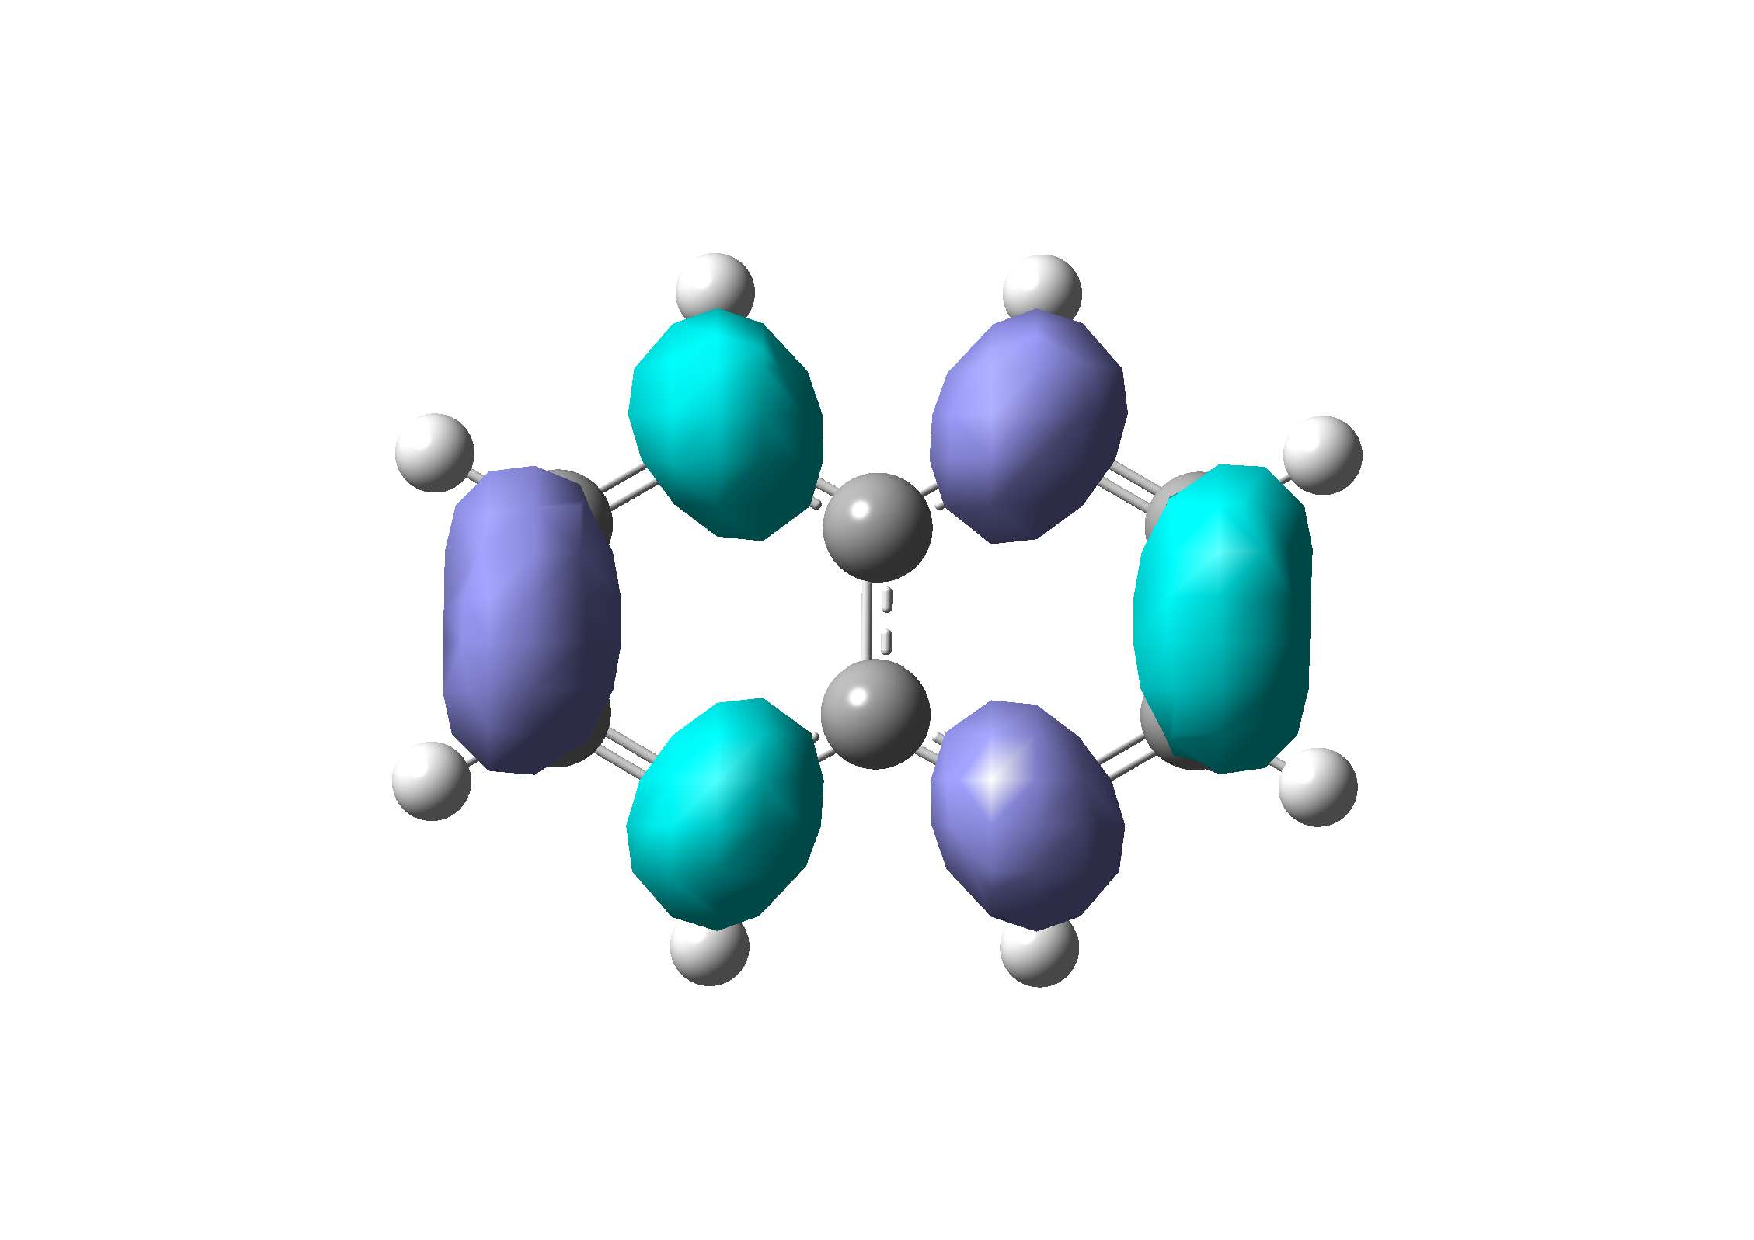
\includegraphics[width=0.45\columnwidth]{Chapters/chap3/Figure4b.pdf}}
\caption{The (a)  ($A_{u}$) HOMO and (b)  ($B_{2g}) $LUMO of naphthalene.\label{naphHOMOLUMO}}
\end{figure*}

\begin{figure*}[]
\subfloat[]{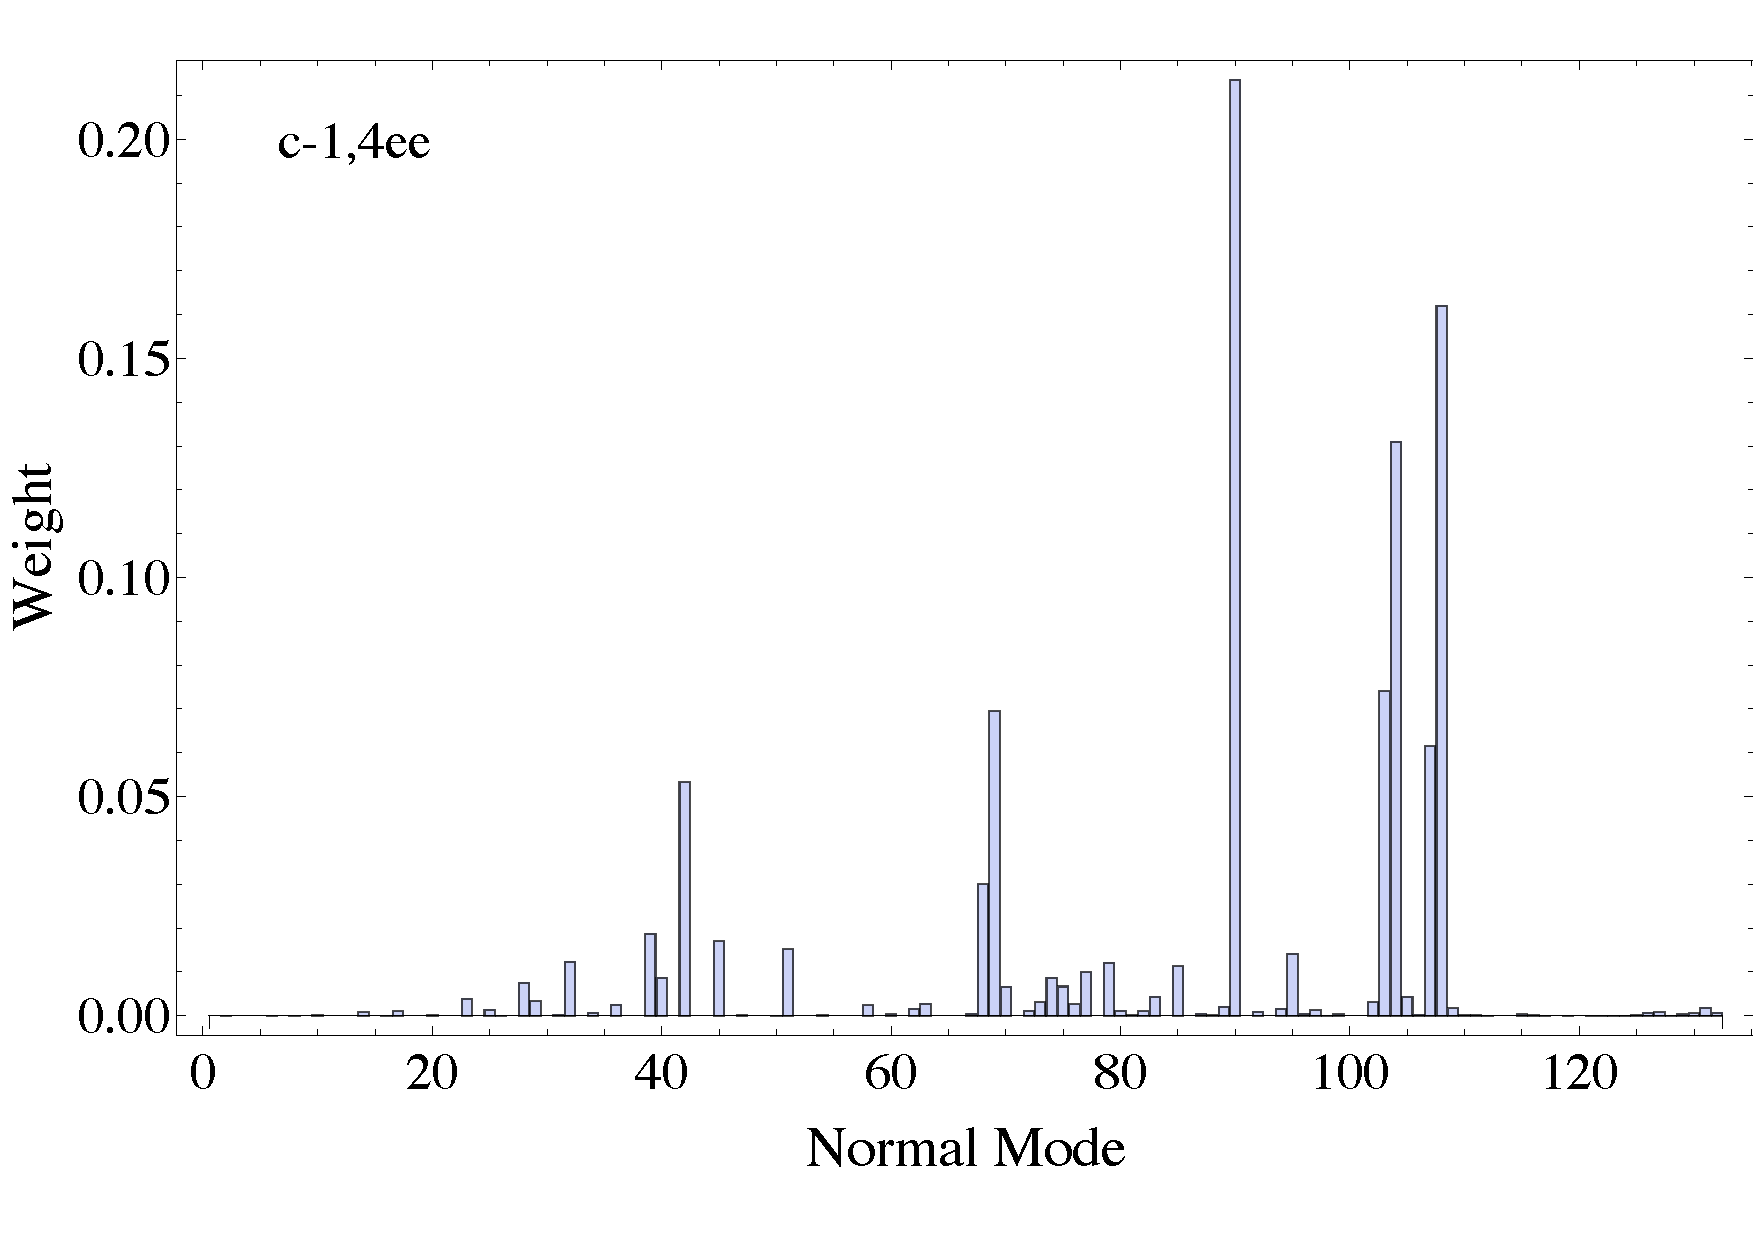
\includegraphics[width=0.82\columnwidth]{Chapters/chap3/Figure5a.pdf}}\\
\subfloat[]{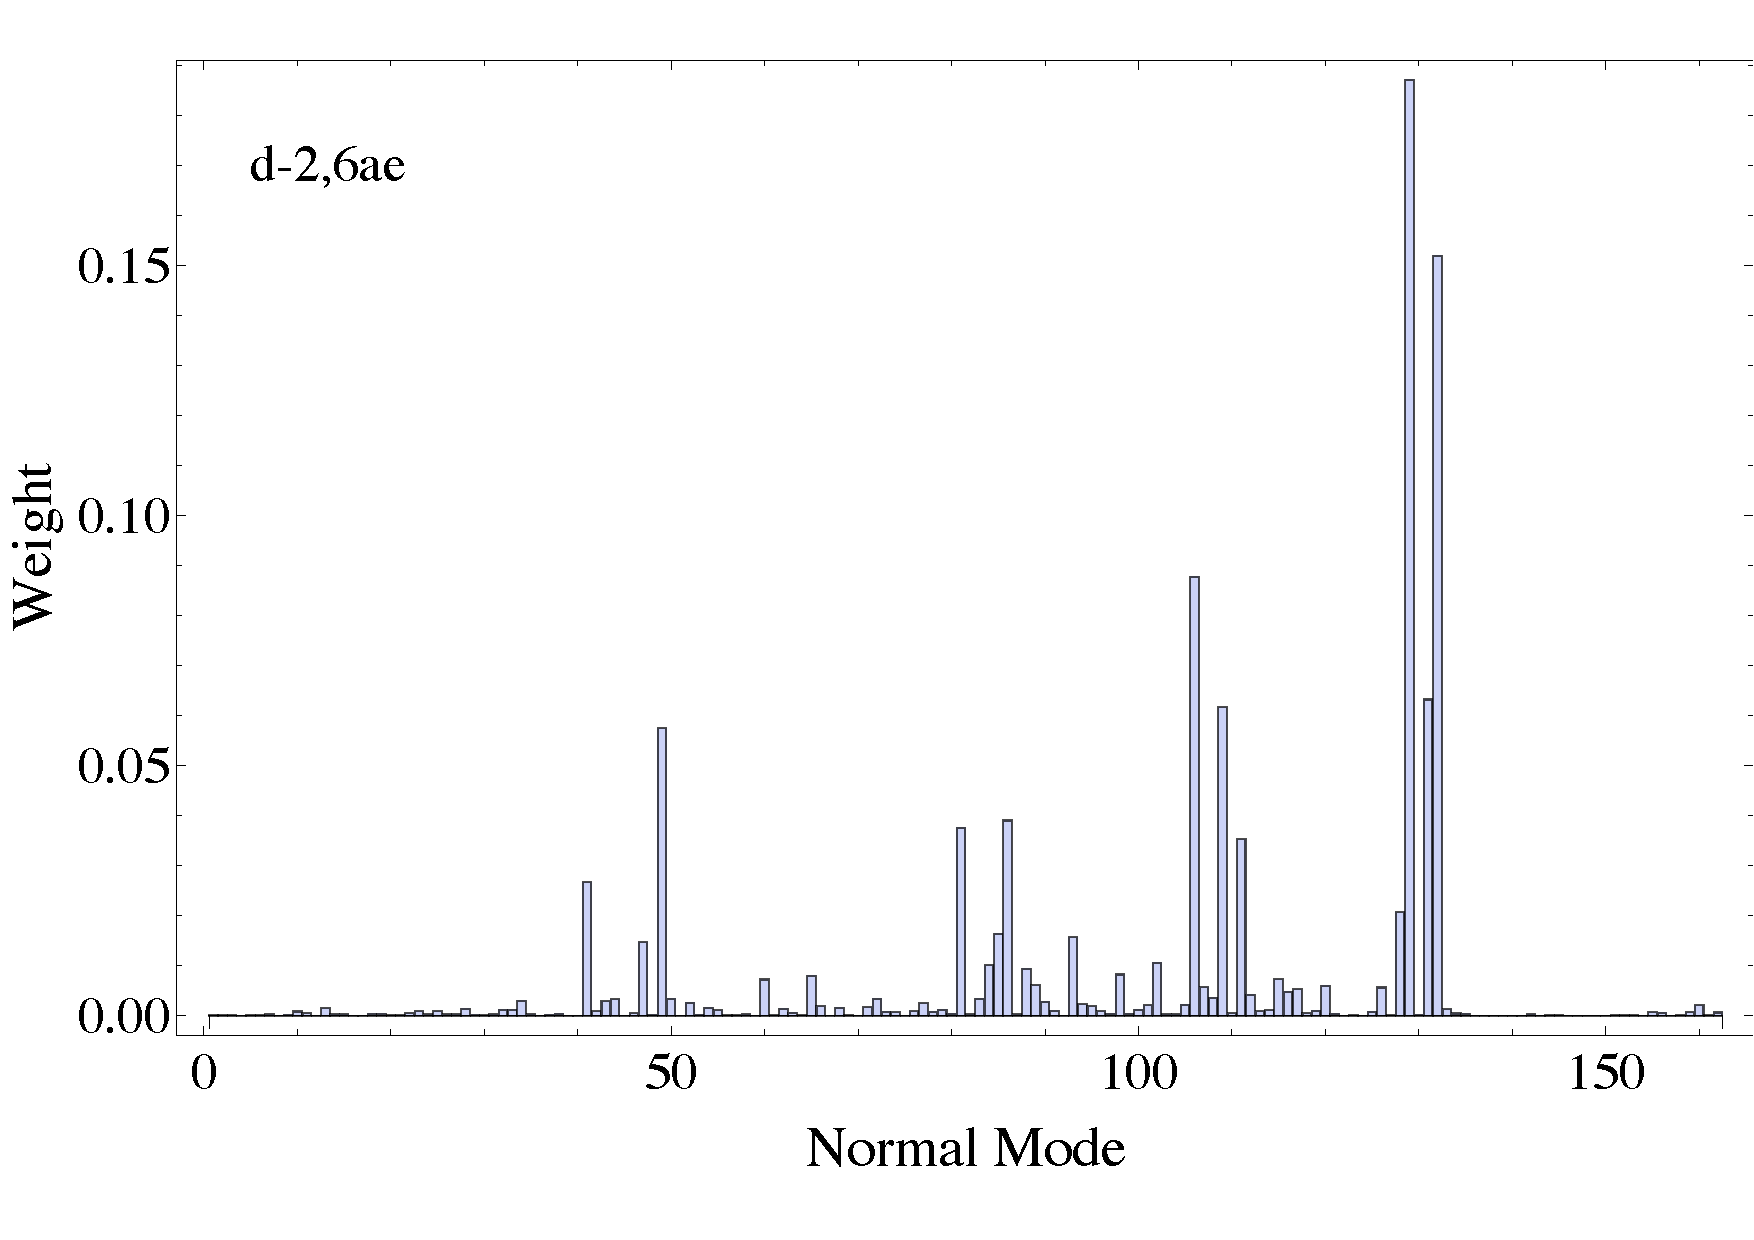
\includegraphics[width=0.82\columnwidth]{Chapters/chap3/Figure5b.pdf}}
\caption{Projections of the PLM onto the normal modes of (a) c-1,4ee and (b) d-2,6ae.\label{LancProj}}
\end{figure*}



%{\bf  Comment: this paragraph needs fleshing out since there's a lot going on here.}
It is not a coincidence that the PLMs belong to the totally symmetric irreducible representation of the isolated donor and acceptor moieties.
This connection can be understood by analyzing the corresponding  the changes in the electron density that accompany the transition.
For example, the PLM on the naphthalene part shown in  Fig.~\ref{LanczosModes_chap2}
largely corresponds to a symmetric ring-stretching mode,  involving carbons
C1 - C2, C3 - C4, C5 - C6, and C7 - C8.
During the exciton transfer, an electron is promoted from the naphthalene HOMO to the naphthalene LUMO (shown in Fig.~\ref{naphHOMOLUMO})
and one expects that changes in the bond lengths should reflect the changes in
electronic population.
For naphthalene, a HOMO$\to$ LUMO transition would
decrease the $\pi$-bond order between C1 - C2, C3 - C4, C5 - C6, and C7 - C8.
%As shown in
%electronic population in the  naphthalene HOMO contributes to the $\pi$ bond-order
%between these atoms while population in the naphthalene LUMO  would decrease
%$\pi$-bonding between C1 - C2, C3 - C4, C6-C7, and C8-C9.
% Since bond length does not depend on the sign of
%electron orbital density, naphthalene changes the geometry in a symmetric way, and
Similar statements can be made for the phenyl and anthracene systems.
In next section,  we examine the PLMs and bond-length changes that occur during an energy  transfer event.
We show that, in a more quantitative way,   while the  PLMs can be understood in terms of
geometric changes in the molecule,  the reverse is not true.
It is not at all straightforward to determine the PLMs by taking the difference between the initial
and final geometries of the molecule.
%{\bf Question:  if you examine the bond-lengths of the Naphthalene anion,  do you see a similar behavior?}


\section{Localized Property of the Primary Lanczos Mode}

We have established  that the primary Lanczos mode is more like the normal modes of the isolated
donor and acceptor moieties, rather than of the entire molecule. The relation between the
PLM and bond length change partially verifies our statement.
In this section, we explore  the localization in greater detail.
First, we project the PLM onto the normal modes of entire molecule,
which is shown in Fig.~\ref{LancProj}, as a comparison to Fig.~\ref{fragProj}, where the normal modes of the individual moieties are used.    It is clear that on the basis of entire molecule, more modes are significantly involved.   This is in contrast to the projection of the PLM onto only the local modes of the isolated moieties, only a handful modes contribute.  Since the PLM  best captures the initial nuclear dynamics,
 its close relation with local sites reveals the fact that the exciton transfer here is more like a local excitation/de-excitation
coupled by exchange interaction,  in accordance with the Dexter mechanism \cite{dexter1953theory}.

\begin{figure*}[]
\subfloat[]{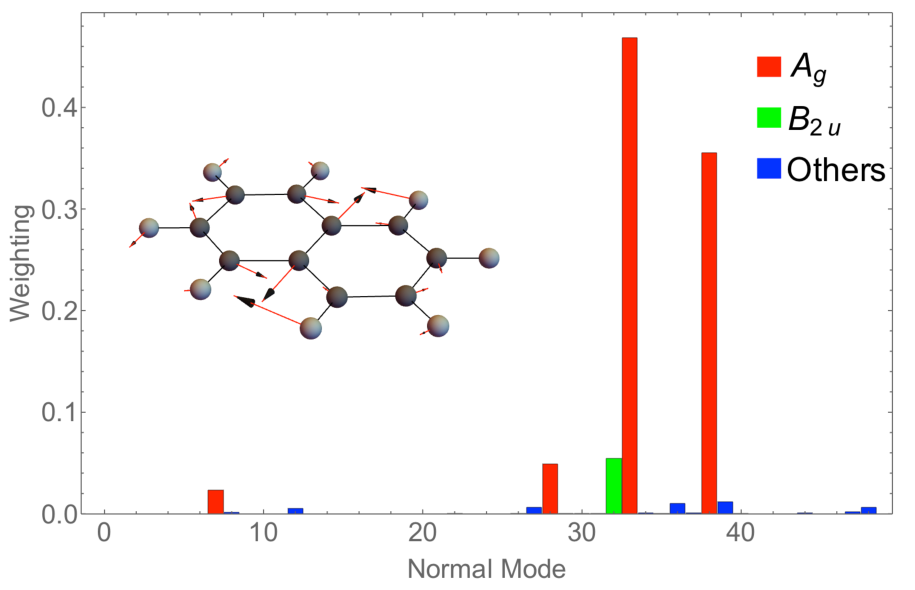
\includegraphics[width=0.78\columnwidth]{Chapters/chap3/Figure6a.pdf}}\\
\subfloat[]{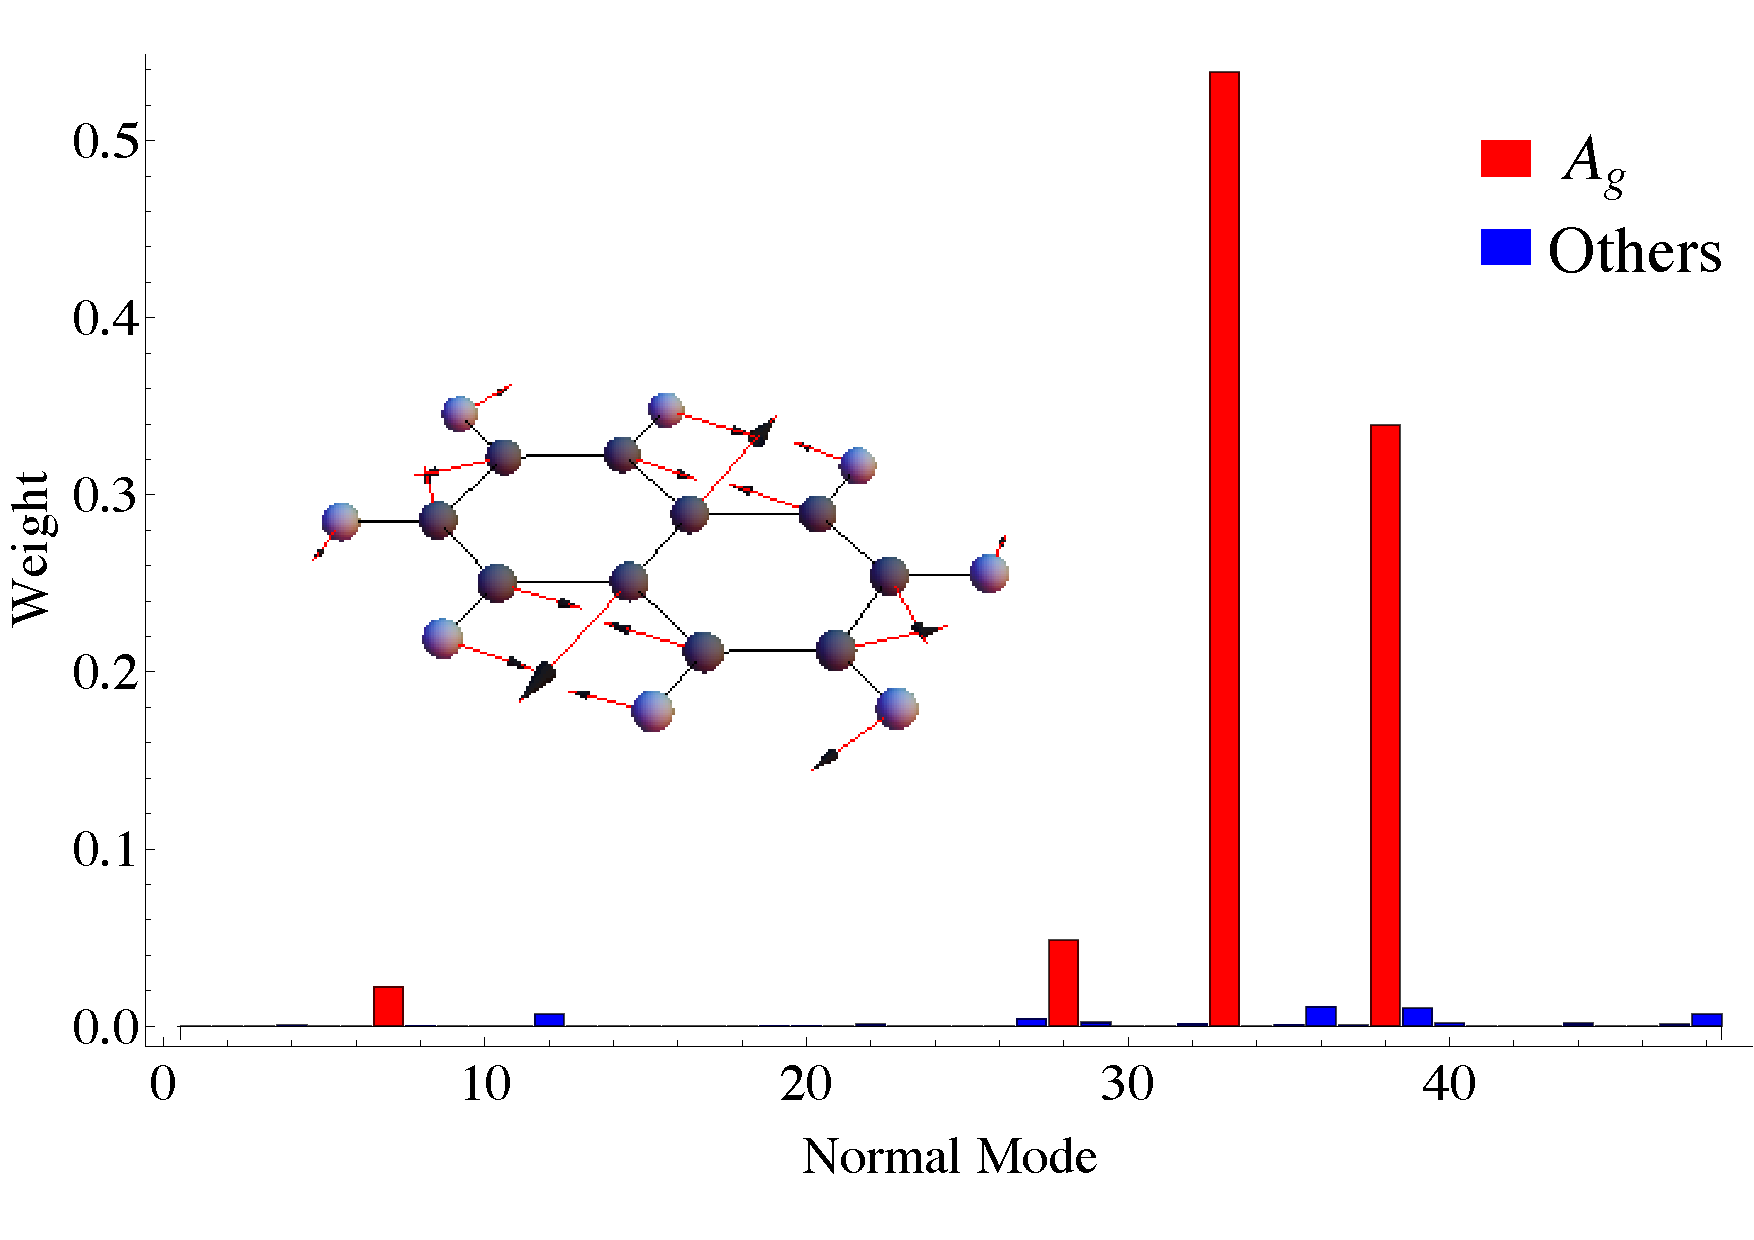
\includegraphics[width=0.78\columnwidth]{Chapters/chap3/Figure6b.pdf}}
\caption{Projection of PLMs onto unsymmetrized naphthalene for (a) c-1,4ee and (b) d-2,6ae.
They are almost same to Fig.~\ref{fragProj}(b) and (d) except for a mode with $B_{2u}$ symmetry in c-1,4ee.
Embedded are the most significant modes, namely, the 33rd modes \label{projNaph}}
%\subfloat[]{\includegraphics[width=0.45\columnwidth]{Chapters/chap3/C14eeNaphProj.pdf}}
%\subfloat[]{\includegraphics[width=0.45\columnwidth]{Chapters/chap3/D26aeNaphProj.pdf}}
%\subfloat[]{\includegraphics[width=0.45\columnwidth]{Chapters/chap3/c-1,4eeNaph1stMode.png}}
%\subfloat[]{\includegraphics[width=0.45\columnwidth]{Chapters/chap3/d-2,6aeNaph1stMode.png}}
%\caption{Projection of PLMs onto unsymmetrized naphthalene for (a) c-1,4ee and (b) d-2,6ae. They are almost same to Fig.~\ref{fragProj}(b) and (d) except for a mode with $b_{2u}$ symmetry in (c). In the second row are the most dominant mode in projections above, namely, the 33rd normal mode of naphthalene in (c) c-1,4ee and (d) d-2,6ae. The mode in (d) belongs to  $A_g$ representation quite well while in (c), hydrogens move  in the  $B_{2u}$ way. \label{projNaph}}
\end{figure*}


%To construct coupling modes from the projections. We take the normal modes in  Fig.~\ref{projNaph}, starting from the most significant ones, and sum their displacement vectors multiplied by their weights in projection. Results are summarized in Fig.~\ref{backCorr}. Several conclusions can be made here. First, taking all modes in both sites, the ``NfBf'' in graph, gives same correlation function to the exact PLM. It verifies our observation that the bridge unit is negligible in PLM. Secondly, taking one mode in each fragment is not enough. 5 modes in each site is good enough and taking 10 gives indistinguishable correlation functions. Nevertheless, correlation function does not need to coincide perfectly to give a good rate constant so we calculate the rate constants for various combinations up to 10 modes in each fragment. The contour plots of the absolute values of their relative errors compared to the rate of PLM are shown in the second row in  Fig.~\ref{backCorr}. We can see that, roughly, taking 3 modes in benzaldehyde and 2 modes in naphthalene suffices to give rate constants within 10\% error. The fact that more modes are needed in benzaldehyde is because more normal modes in it are involved in PLMs, as can be seen in Fig.~\ref{fragProj}.

% One may argue that bridge is not included in our comparison.
We do not include the bridge in the projections, because as showed in Fig.~\ref{LanczosModes_chap2}, very few motions involving the bridge contribute to the PLM.
Thus, we anticipate that we can construct the PLM using only local modes on the donor and acceptor units.
 In the next section, we  quantitatively verify this by using only
dominant modes on the  donor and acceptor to construct coupling modes.

%----- THIS PARAGRAPH IS A BIT CRYPTIC--------
However, before we can compare different ways to construct the Lanczos modes, we first need to
address a  subtle problem.   In the previous section, we symmetrized the geometry of naphthalene
for the convenience in assigning  irreducible representations to the vibrational modes.
However, for constructing the modes
for the entire unit one needs to use the optimized rather than symmetrized geometry.
In Fig.~\ref{projNaph}  we show the project of the PLM onto the modes for optimized
naphthalene.  The irreducible representations have been roughly assigned to the dominant modes.
%Since we did not symmetrize benzaldehyde, its projection remains same.
The projections are
almost same to the ones on the symmetrized geometry, except a new $B_{2u}$ mode is involved
in c-1,4ee. However, it does not exist in d-2,6ae. The reason is that the most significant
mode of c-1,4ee and d-2,6ae are slightly different. The corresponding displacement vectors are
embedded in Fig.~\ref{projNaph}. For c-1,4ee, the dominant mode is not an exact $A_g$ mode, because
carbons move in the way of $A_g$ while
hydrogens behave like $B_{2u}$. On the contrary, d-2,6ae has
a mode more similar to $A_g$.
As the result, in the projection of naphthalene in c-1,4ee, a  $B_{2u}$
mode is needed to correct the hydrogen motions.

To construct coupling modes, we collect a small number of modes on both naphthalene
and benzaldehyde in the order of decreasing weights, then sum up the displacement vectors
multiplied by their weights.
We then bench-mark the quality of taking various different  combinations
of normal modes by computing the coupling auto-correlation function in  Eq. 3 and comparing to
the exact result obtained by including all modes.
We denote these as N$x$B$y$ where $x$ denotes the number of naphthalene  local modes and $y$ denotes
the number of benzaldehyde  local modes used in each case.
NfBf denotes that {\em all} local modes are
included.   The correlation functions and rate constants derived from various
combinations of normal modes are summarized in Fig.~\ref{backCorr}.


\begin{figure*}[!h]
\subfloat[]{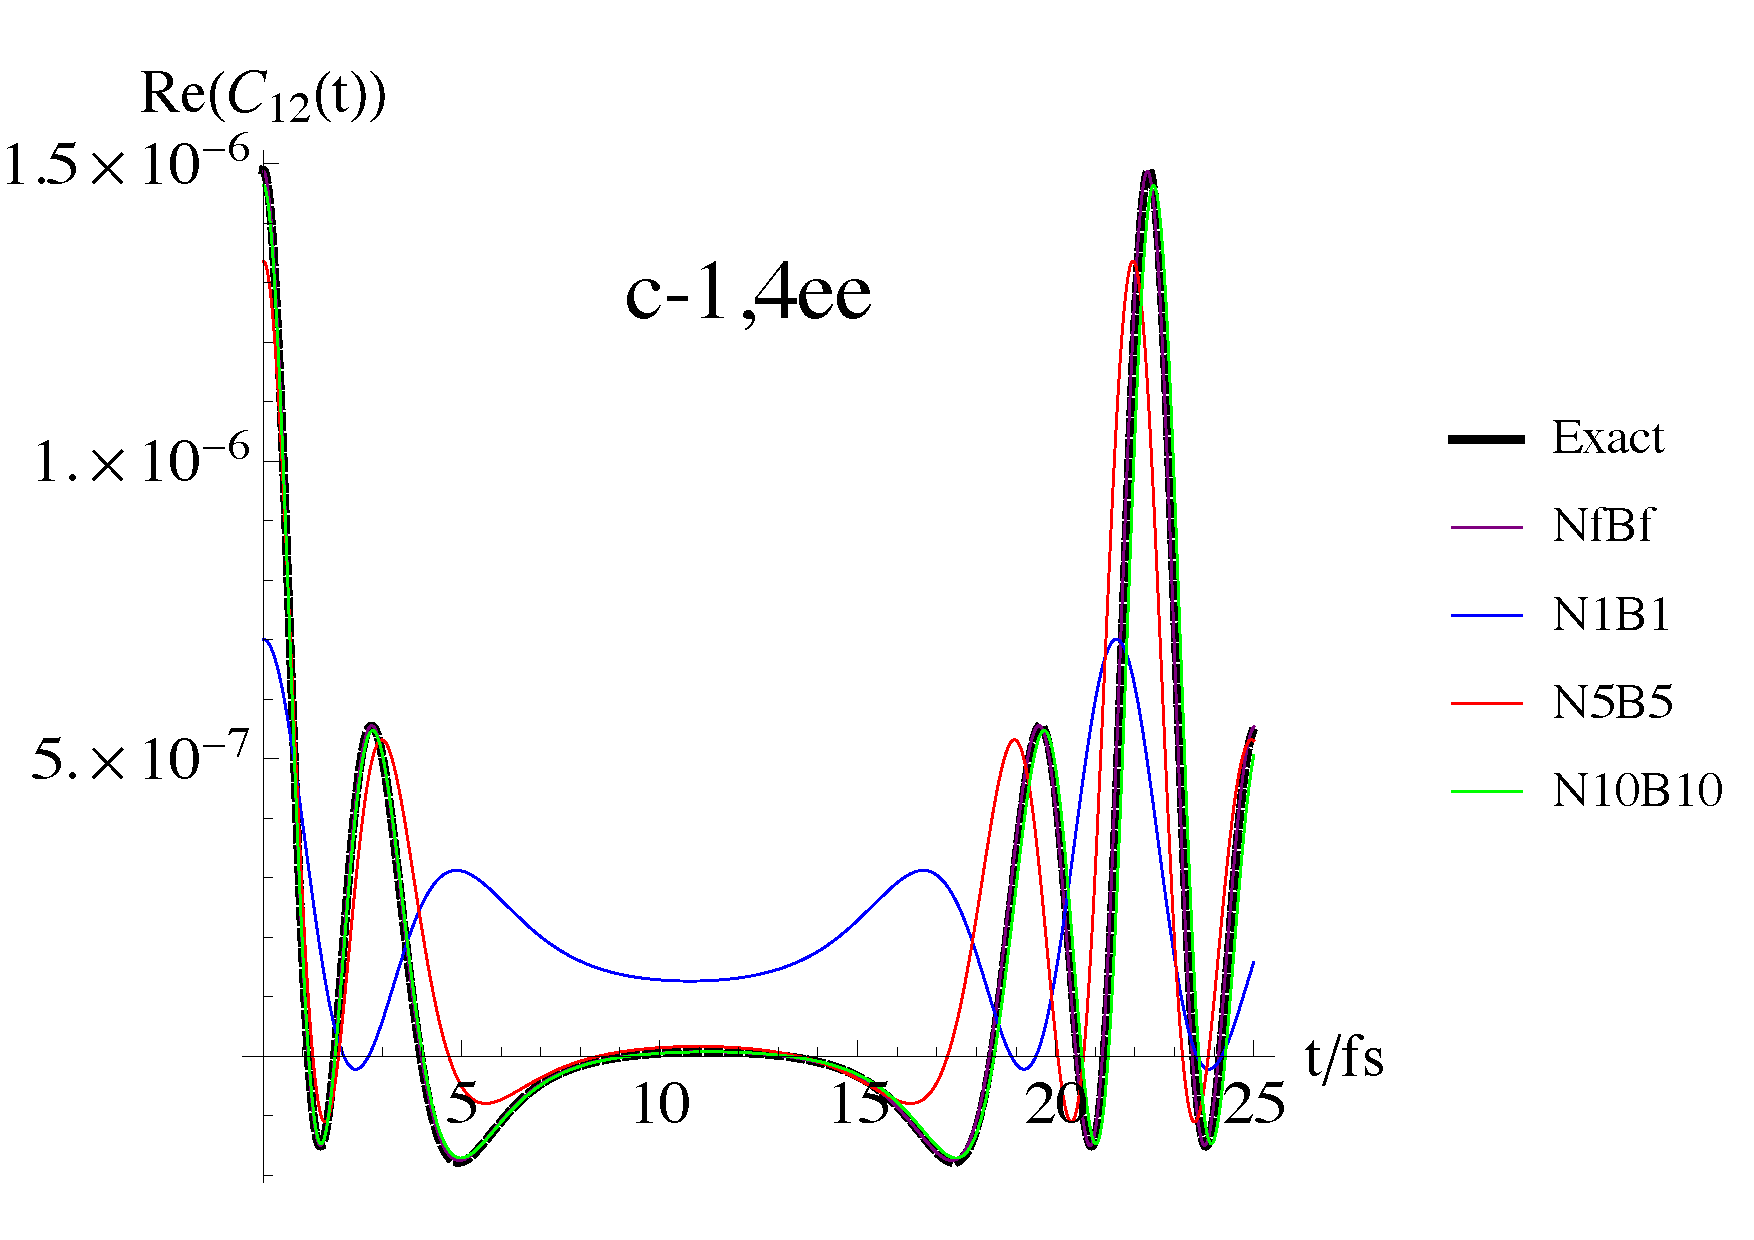
\includegraphics[width=0.5\columnwidth]{Chapters/chap3/Figure7a.pdf}}
\subfloat[]{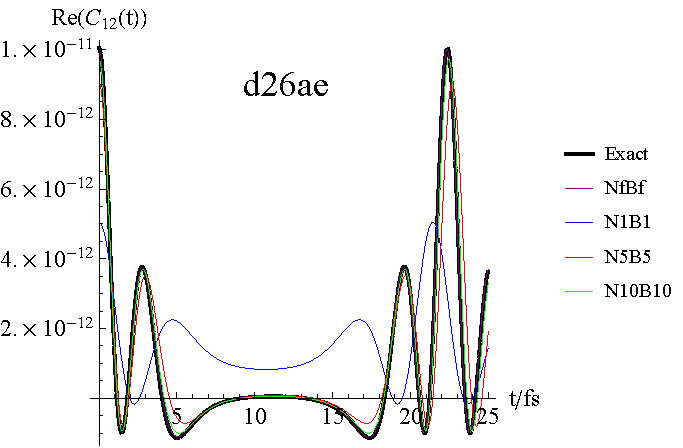
\includegraphics[width=0.5\columnwidth]{Chapters/chap3/Figure7b.pdf}} \\
\subfloat[]{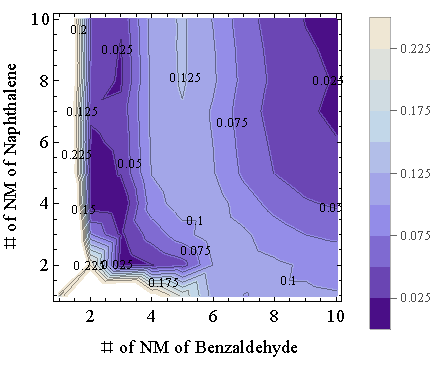
\includegraphics[width=0.5\columnwidth]{Chapters/chap3/Figure7c.pdf}}
\subfloat[]{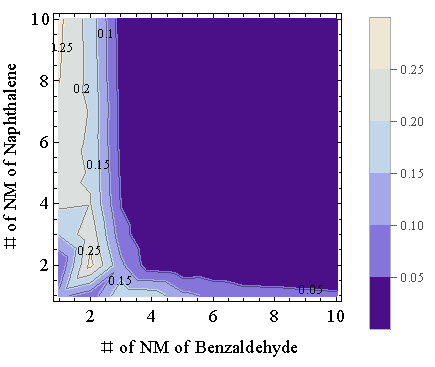
\includegraphics[width=0.5\columnwidth]{Chapters/chap3/Figure7d.pdf}}
%\subfloat[]{\includegraphics[width=0.45\columnwidth]{Chapters/chap3/backrateC14ee.pdf}}
%\subfloat[]{\includegraphics[width=0.45\columnwidth]{Chapters/chap3/backrateD26ae.pdf}}
\caption{Correlation functions for different combinations of normal modes are shown for (a) c-1,4ee and (b) d-2,6ae.  The ``exact'' ones refer are for the PLMs.  ``NfBf"
is the mode made up from all normal modes of both the donor and acceptor sites.
The designation ``NxBy'' indicates that the correlation function was constructed using  $x$ most significant normal modes
on naphthalene and $y$ most significant ones on benzaldehyde.   Plots (c) and (d) show the
 relative error in rate constants calculated for various combinations of normal modes compared to the exact result
 of c-1,4ee (c) and d-2,6ae (d), respectively. \label{backCorr}}
\end{figure*}


 First, if we take all local modes from both moieties, (NfBf)
 the resulting approximated correlation function is indistinguishable from the exact correlation function.
This verifies our observation that the bridge unit is not needed in constructing the
PLM.
%Secondly, taking one mode in each moiety is not enough. 5 modes in each is good
%enough and taking 10 gives almost perfect correlation functions.
In order to achieve adequate agreement with the exact correlation function,
at least 10 of the strongest contributing local modes are needed from both the donor and acceptor units.
%Furthermore, as shown

However, as seen on our previous work \cite{yang2014intramolecular},
the approximate correlation function does not need to give perfect agreement
with the exact correlation function to produce an accurate transition rate constant (Eq. 4).
To assess the accuracy of using different combinations of local modes,
we calculate the transition rate constants for various combinations up to 10 modes on
each moiety and compare to the exact rate.
This data is summarized in the form of contour plots in  Fig.~\ref{backCorr}(c,d).
For the c-1,4ee case, there is an optimal ``valley'' whereby taking 3 modes from benzaldehyde and 4-6 modes from
naphthalene produces an agreement with the exact result to within 5\%.
For the d-2,6ae case,  fewer number of benzaldehyde modes than naphthalene modes are needed to
give agreement to within 5\% of the exact rate constant.   This is easily anticipated since
naphthalene is simply a larger molecule with more normal modes.


\section{Geometry Change and Relaxation Mode}

We showed that the PLMs agree with bond length changes on the moieties.   We next
consider the relation between the PLM and geometry change accompanying the transition.
First, we use the PLM to approximate geometry change by distorting the molecule
along the PLM.   The magnitude of the distortion
 is determined  by minimizing the average bond length difference of the four bonds on naphthalene
 which stretch significantly in PLM, between the optimized and approximate geometries. In Table. ~\ref{aprroxGeom} we list the differences between two geometries.
Comparing the maximum difference of bond
lengths and angles between the approximated and true final states, the differences are very small,
so PLMs seem to give fairly good approximations of geometry changes.


% We will then compare the projection of geometry change to that of the PLM.
% They seem to contradict each other. We conclude that the apparent contradiction
% reveals the mechanism of the transfer reaction, which is consist of two steps, agreeing with
% the Born-Oppenheimer principle.

\begin{table*}[t]
 \caption{Approximated geometry using the PLM and the relaxation modes (RM) compared to acceptor states}
 \label{aprroxGeom}
 \begin{tabular}{lllll}
   \hline
   Mode used & c-1,4ee-PLM   & c-1,4ee-RM  & d-2,6ae-PLM  & d-2,6ae-RM\\
   \hline
   Max. bond length difference (\AA)   & 0.034 & 0.160 &0.039 & 0.283   \\
     Max. bond angle difference (rad)   & 0.053 &0.075 & 0.057 &0.135   \\
   \hline
 \end{tabular}
\end{table*}


%
%First we add PLM with a magnitude to initial donor state geometry,
%to get an approximate geometry of final state.
%In Table. ~\ref{aprroxGeom} we list the maximum difference of bond
%lengths and angles between the approximated and real final states. The differences are small,
%so PLMs seem to give fairly good approximations of geometry changes.
%In this part we discuss the mechanism why PLM is totally symmetric in donor and acceptor moieties. We show that it corresponds to geometry change of the moieties in the transfer. However, simply taking the difference of coordinates of initial and final states does not give PLM. By breaking down geometry change, we get the insight that the entire process consists of two steps, the fast excitation transfer facilitated by PLM and the relaxation after that.
%Looking at the symmetry of PLM in Fig.~\ref{LanczosModes_chap2}, especially the naphthalene, it is basically the stretch of four bonds being symmetric to each other. Comparing the bonding and antibonding in the HOMO/LUMO of naphthalene in Fig.~\ref{naphHOMOLUMO}, we noticed that these four bonds change lengths dramatically in deexcitation, so does PLM correspond to geometry change? Yes, and no. First, we prove the "yes".



%By adding  PLM with a magnitude to initial donor state, we can get an approximated geometry to final acceptor state. The magnitude is decided by minimizing the average bond length difference of the four bonds in naphthalene mentioned above, between real acceptor state and the approximated one. In Table. ~\ref{aprroxGeom} we list the maximum difference of bond lengths and angles between the derived and real final states. The differences are small. PLM seems to give fairly good approximation of final state geometry.



However, this is only one side of the story and we  need try to do this in reverse, {\em i.~e.}, can we
determine the PLM from simply geometric changes accompanying the transition? To see if this is possible,
we can project the geometry change onto the normal modes of molecule and moieties respectively.  The
results for our two test cases are shown  in Fig.~\ref{geomDiffFragProj} and \ref{geomDiffProj}.



\begin{figure*}[!h]
\subfloat[]{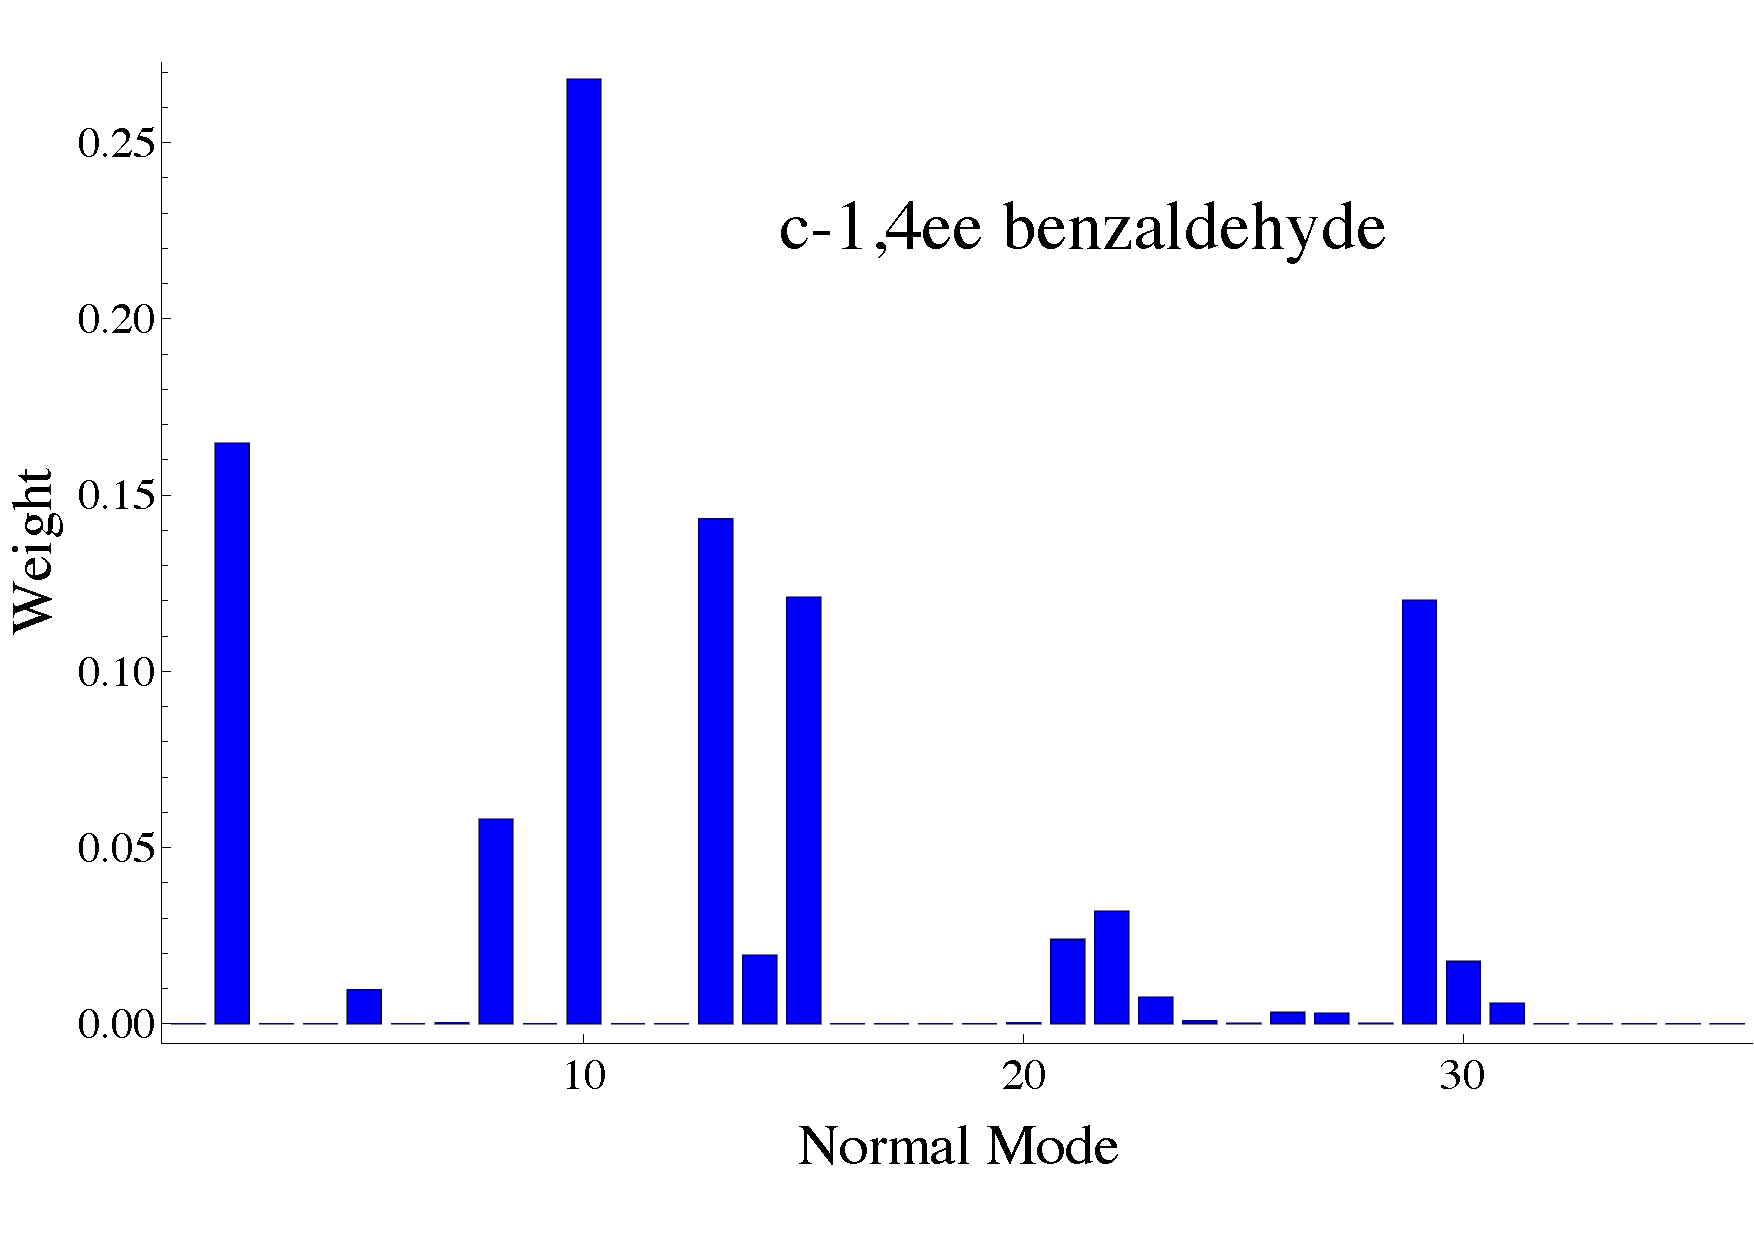
\includegraphics[width=0.45\columnwidth]{Chapters/chap3/Figure8a.pdf}}
\subfloat[]{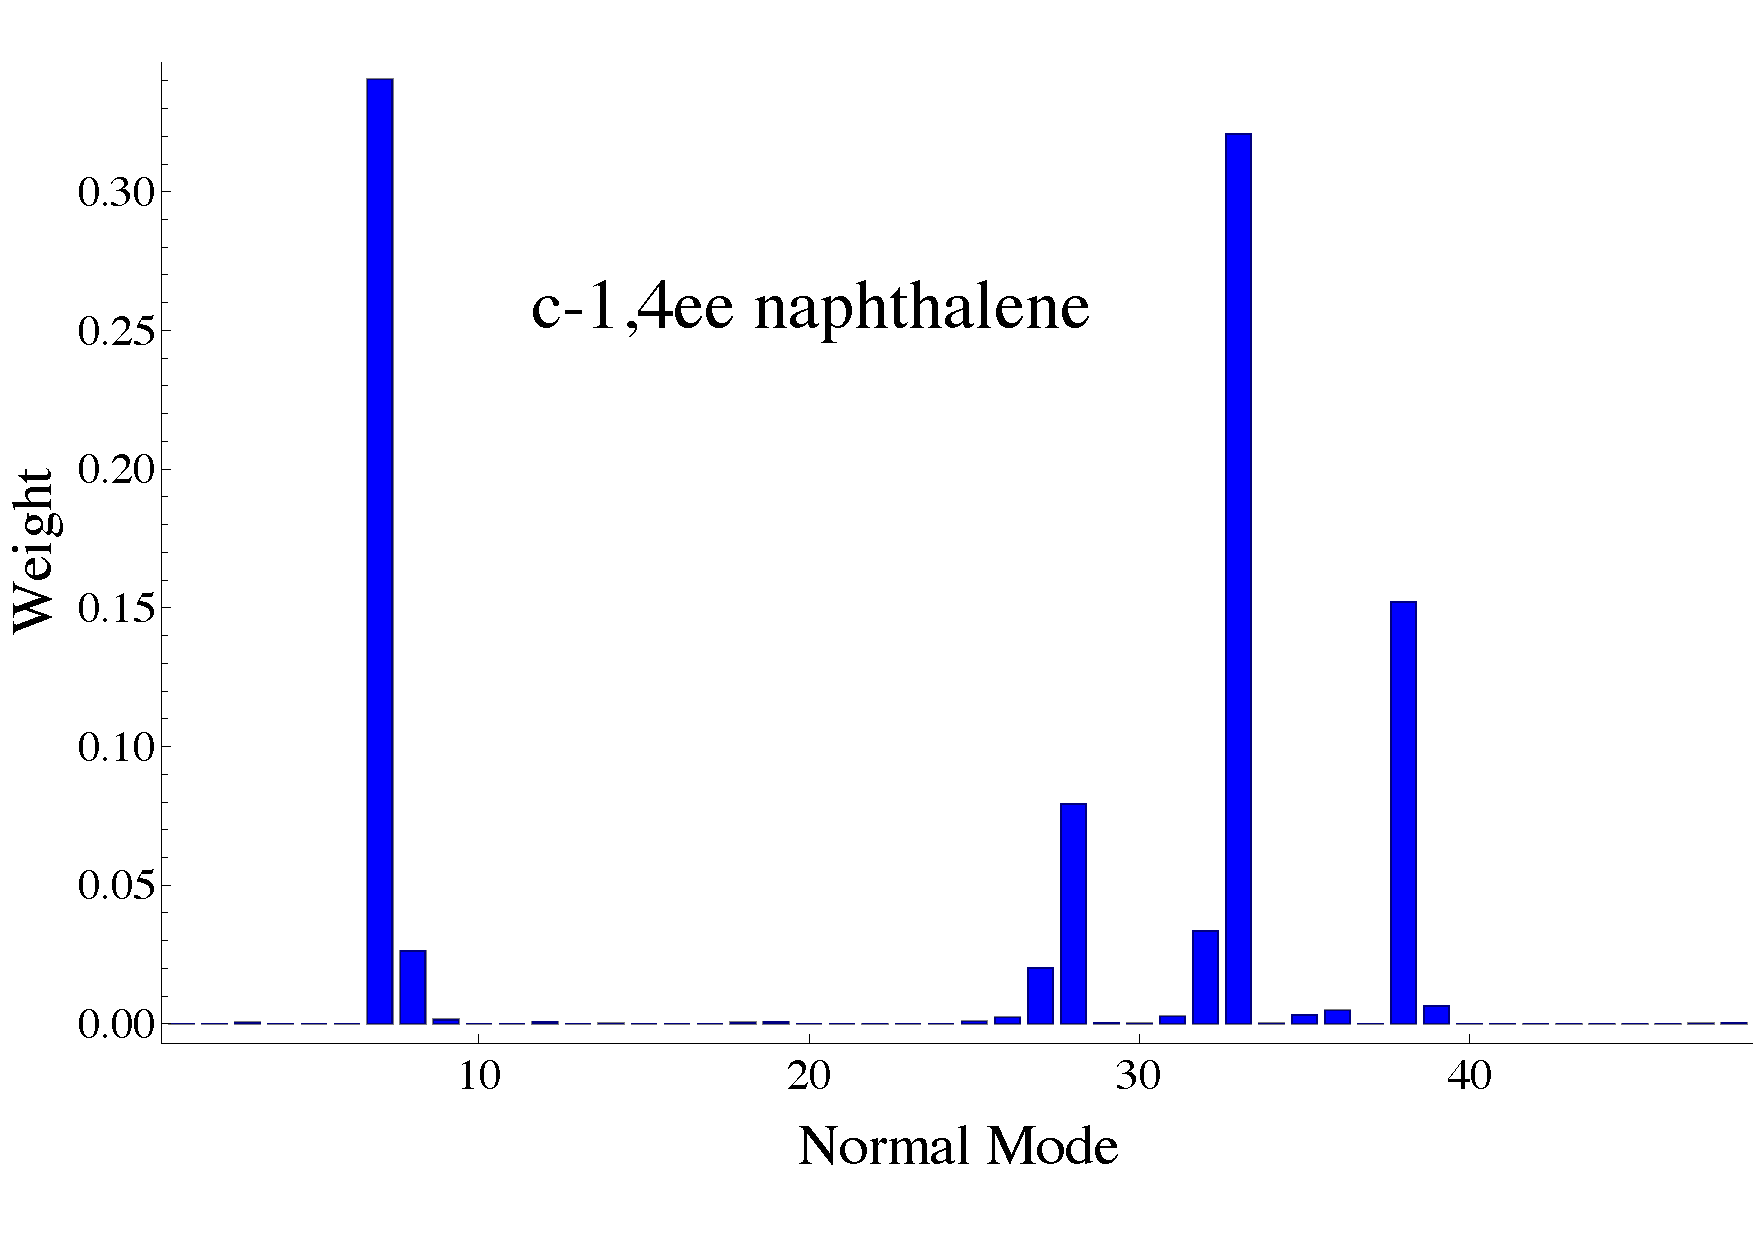
\includegraphics[width=0.45\columnwidth]{Chapters/chap3/Figure8b.pdf}}\\
\subfloat[]{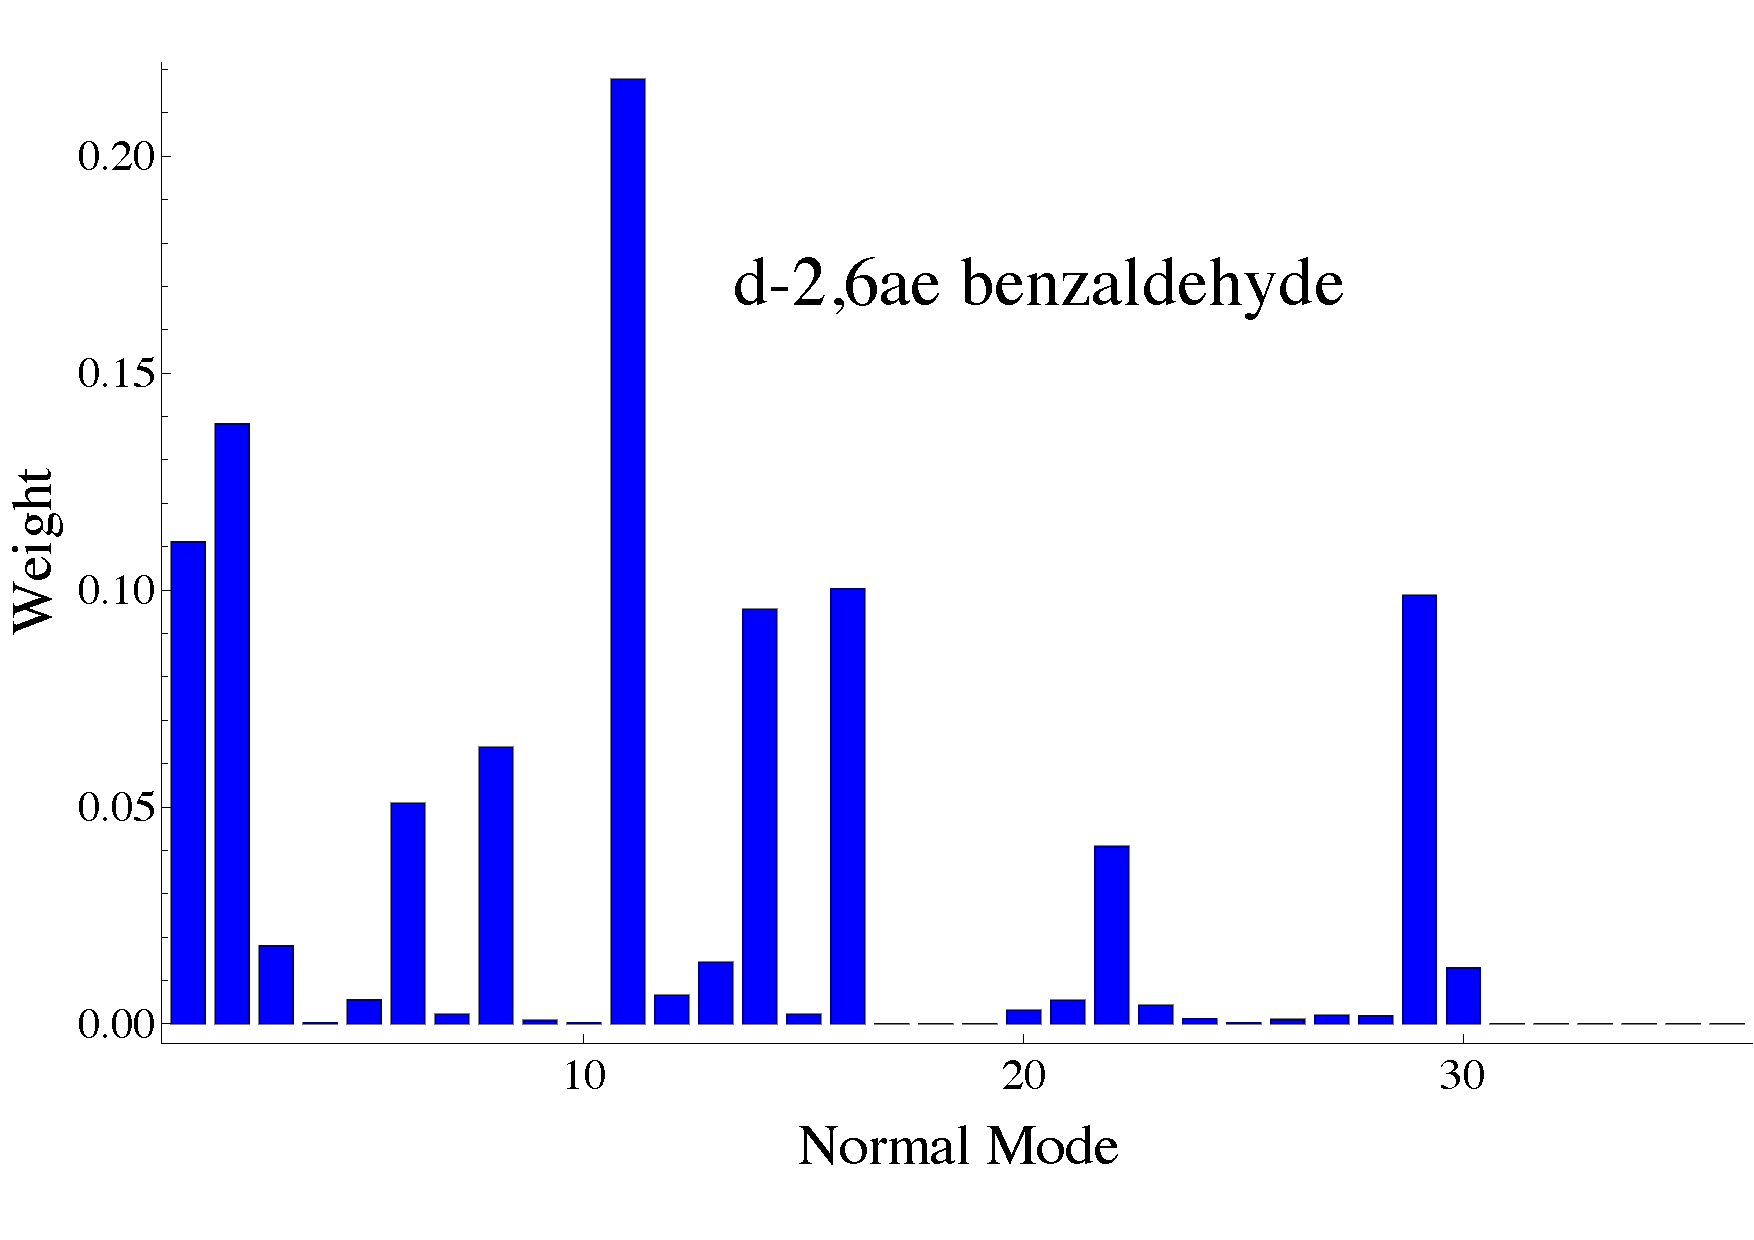
\includegraphics[width=0.45\columnwidth]{Chapters/chap3/Figure8c.pdf}}
\subfloat[]{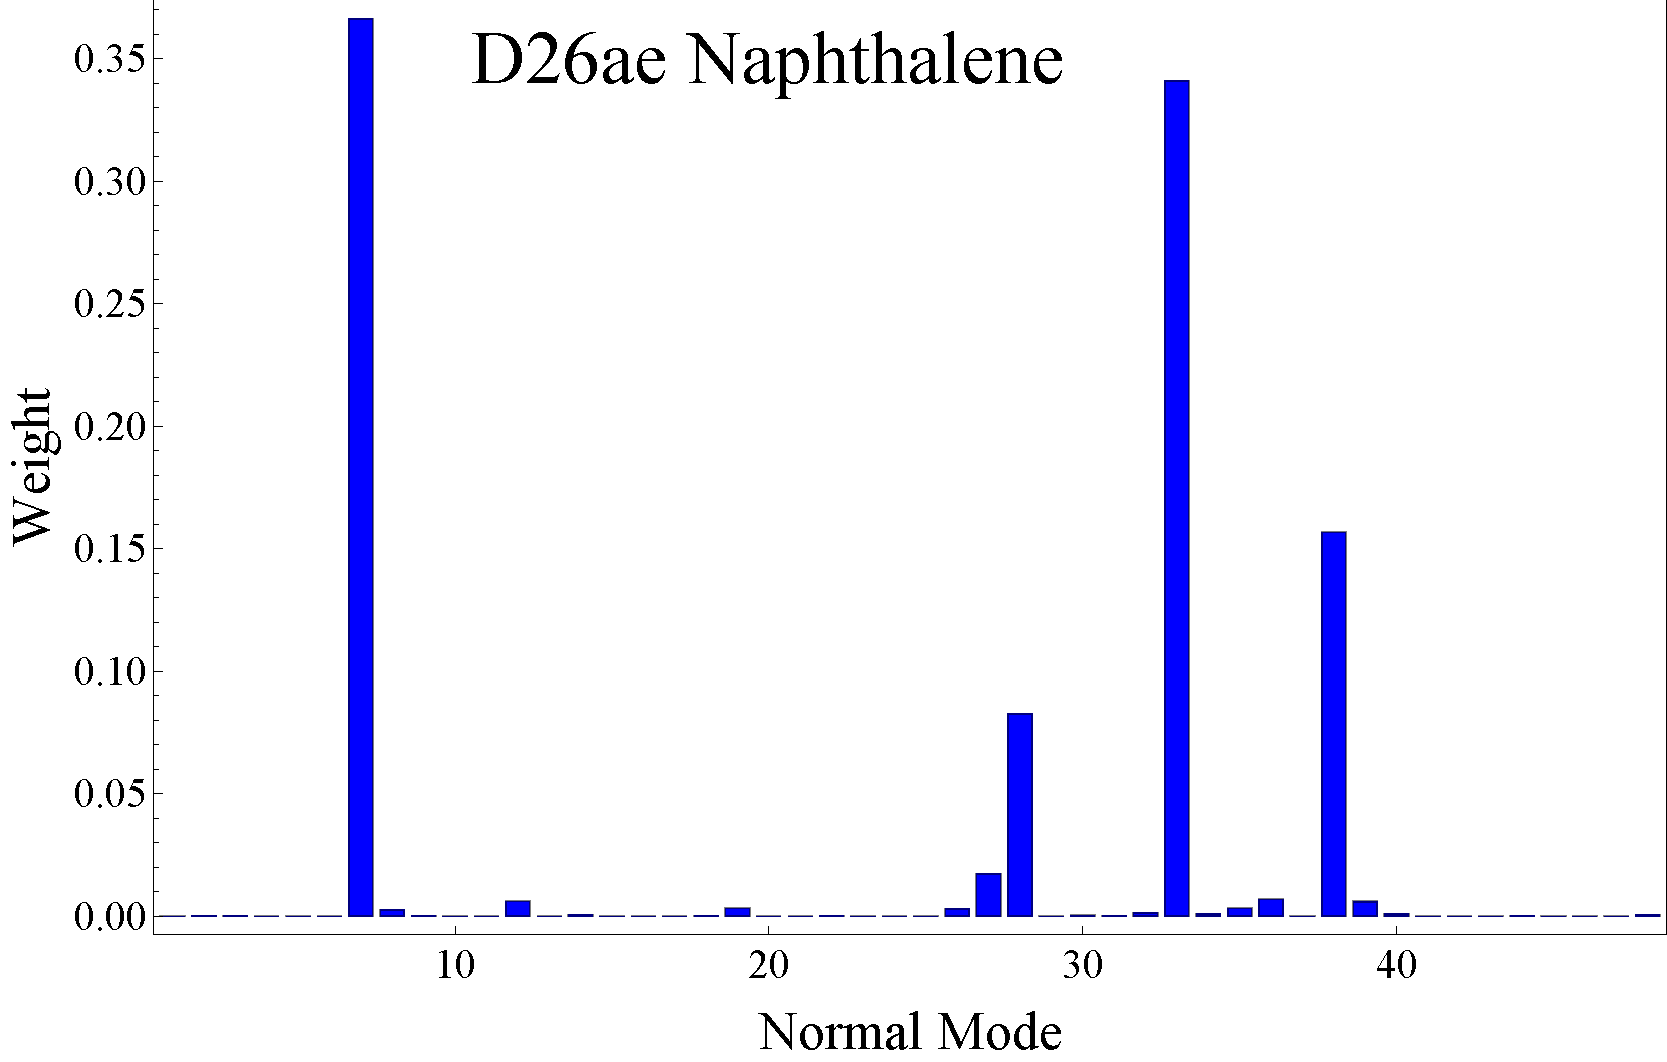
\includegraphics[width=0.45\columnwidth]{Chapters/chap3/Figure8d.pdf}}
\caption{Projections of the geometry change between initial and final states onto the normal modes of (a) benzaldehyde and (b) naphthalene sites in c-1,4ee, and d-2,6ae in (c) and (d). Except for some low frequency modes, they are similar to the projections of PLM. \label{geomDiffFragProj}}
\end{figure*}


\begin{figure*}[]
\subfloat[]{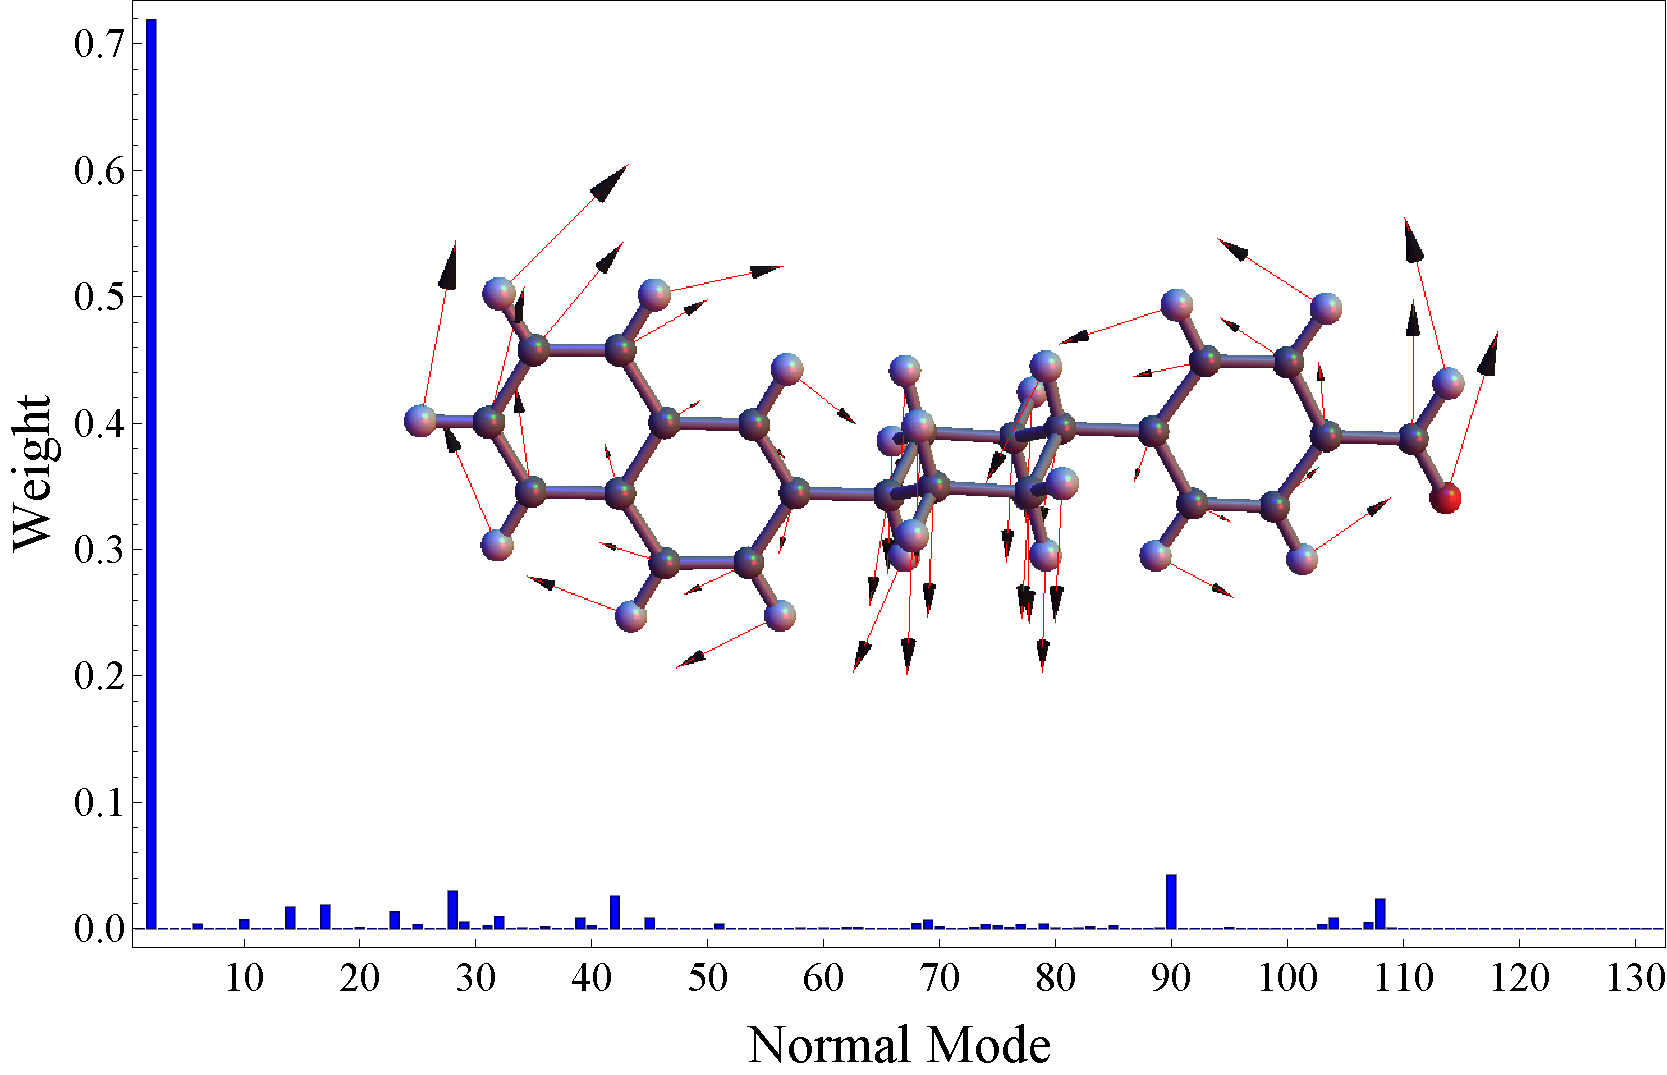
\includegraphics[width=0.82\columnwidth]{Chapters/chap3/Figure9a.pdf}}\\
\subfloat[]{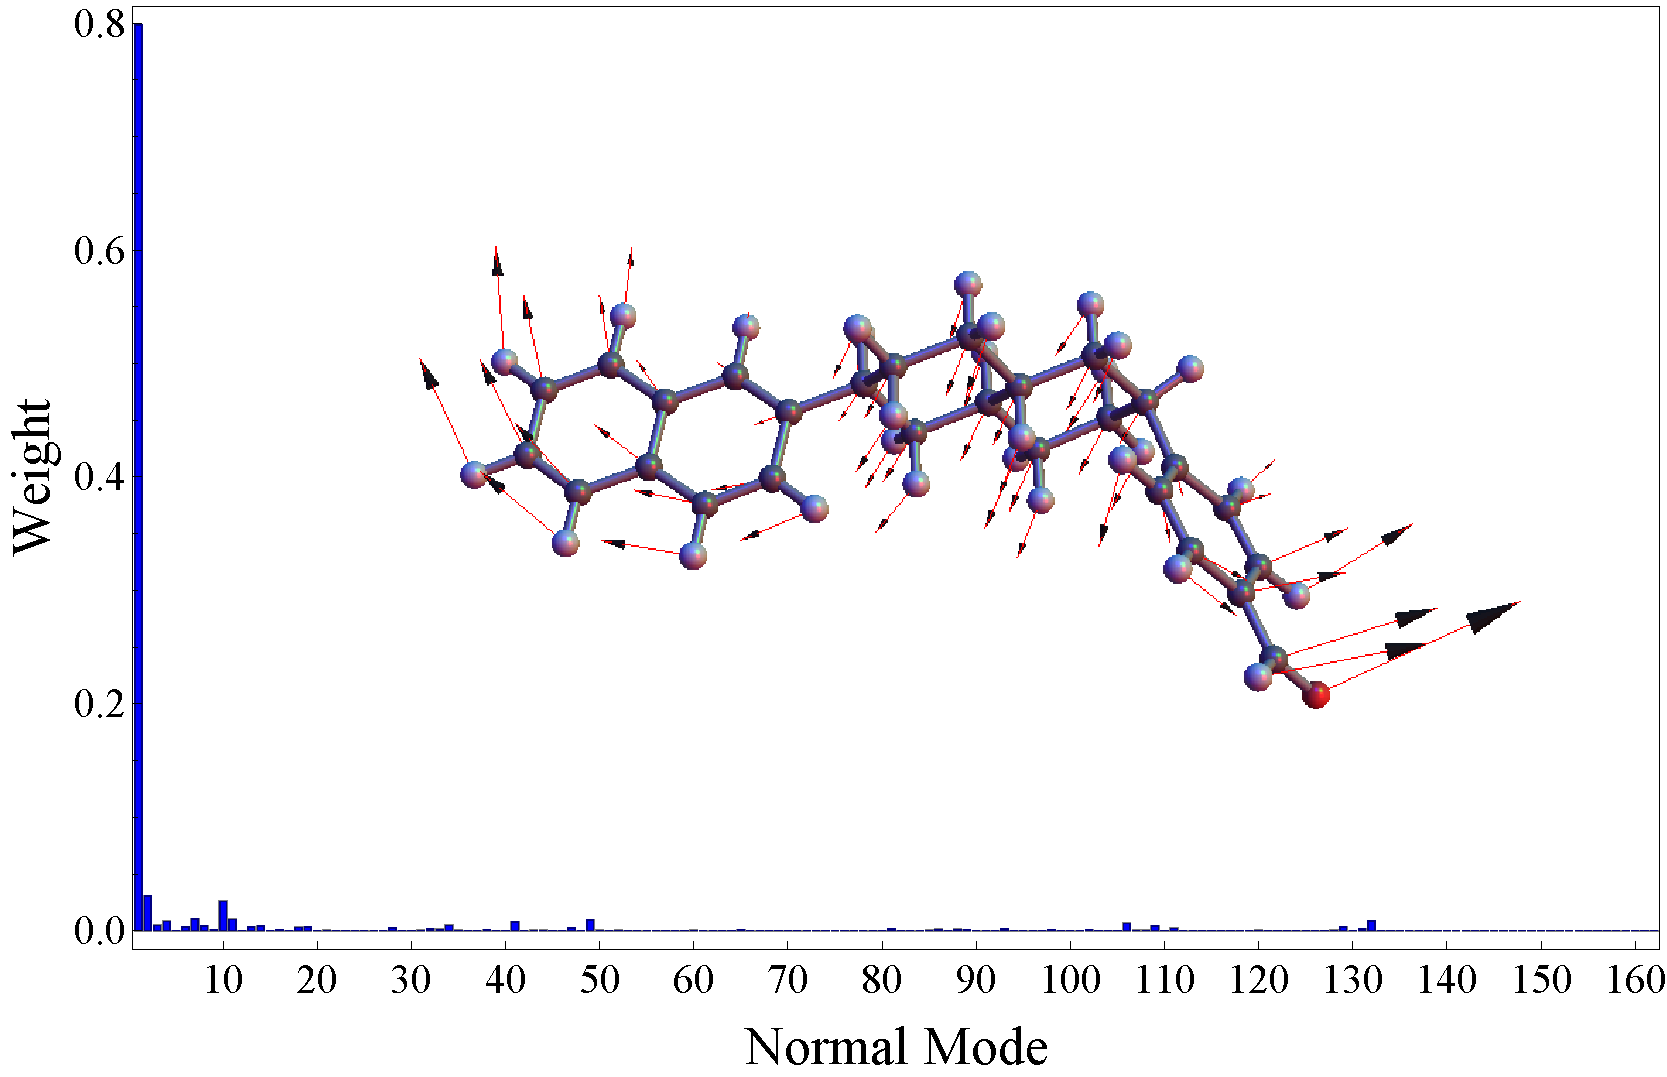
\includegraphics[width=0.82\columnwidth]{Chapters/chap3/Figure9b.pdf}}
%\subfloat[]{\includegraphics[width=0.45\columnwidth]{Chapters/chap3/c-1,4eeDADiffproj.pdf}}
%\subfloat[]{\includegraphics[width=0.45\columnwidth]{Chapters/chap3/d-2,6aeDADiffproj.pdf}}
%\subfloat[]{\includegraphics[width=0.45\columnwidth]{Chapters/chap3/c-1,4eeNM2.png}}
%\subfloat[]{\includegraphics[width=0.45\columnwidth]{Chapters/chap3/d-2,6aeNM1.png}}
\caption{Projections of the geometry change between initial and final states onto the normal modes of (a) c-1,4ee and (b) d-2,6ae. They are both dominated by single mode, the relaxation mode (RM), which is embedded.\label{geomDiffProj}}
\end{figure*}



When projected onto the whole molecule, we see that geometry change is mostly dominated
by one  very low frequency mode  corresponding to an internal  torsion of the entire donor-bridge-acceptor molecule.
Compared to the PLMs in the same basis in Fig.~\ref{LancProj}
 we see that  PLMs  have many more modes involved.
However, if we compare the projections onto the  moieties in  Fig.~\ref{fragProj}
and \ref{geomDiffFragProj}, the geometry changes resemble PLMs well, except in the low frequency region.
In essence, simply changing representation completely changes the implied dynamics.

% \begin{table*}[bh]
%   \caption{Miscellaneous single mode rate constants compared to exact ones}
%   \label{rates}
%   \begin{tabular}{lllll}
%     \hline
%     Mode(s) used &  All NM  & PLM  & Geometry change (GC) & GC without RM component\\
%     \hline
%     Rate constants in c-1,4ee/$s^{-1}$   & 3.66E9 & 3.69E9 & 5.28E9 & 4.31E9   \\
%     Rate constants in d-2,6ae/$s^{-1}$   & 4.66E4 &4.80E4 & 1.30E4 & 5.11E4 \\
%     \hline
%   \end{tabular}
% \end{table*}

%However, this is only one side of the story. In Fig.~\ref{geomDiffProj} we project geometry change onto the normal modes of molecule. It does not look same to the projections of PLM in Fig.~\ref{LancProj}. The geometry change of both c-1,4ee and d-2,6ae are dominated by single mode with very low frequency, shown in Fig.~\ref{geomDiffProj}(c) and (d). We term them the dominant mode relaxation mode (RM) for the reason below. RM does not resemble PLM at all.


The solution to this inconsistency is to distinguish between the two types of geometric changes.
One is the internal changes within  the moieties.  These are well represented  by the PLM.
The other is the gross motion of the entire molecule, which we shall refer to as the ``relaxation mode'' (RM).  This latter motion
is not well represented by the PLM.
%Bond length change belongs to the first type while the relaxation modes
%correspond to the second, as suggested by the orientation of displacement vectors and the low frequency.
 These two kinds of motion  correspond to two different steps that accompany the electronic  transition. The
internal motion primarily affects C=C bond lengths,  and
hence is strongly coupled to the $\pi$-electronic degrees of freedom, while gross motion of moieties corresponds
to  relaxation after exciton transfer has occurred. This is verified in Table 1, where we use the relaxation mode to approximate the final geometry. The procedure is similar to that of PLM. Although RM is the dominant mode in the projection, it gives much worse approximated bond lengths and angles.
% In short, the PLM is a subvector within the relaxation mode.

\begin{figure*}[]
\subfloat[]{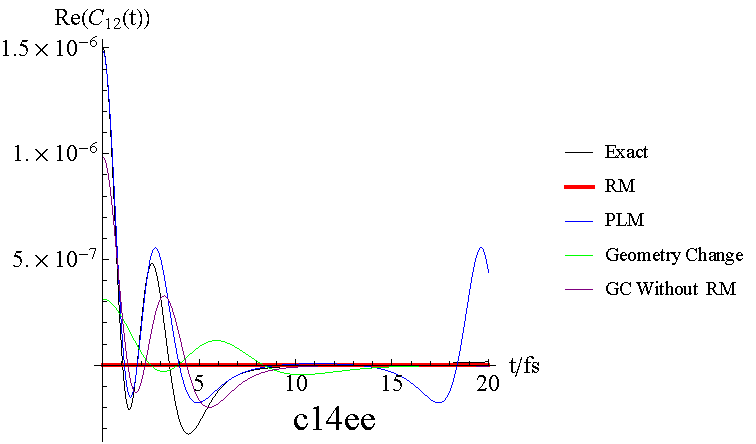
\includegraphics[width=0.78\columnwidth]{Chapters/chap3/Figure10a.pdf}}\\
\subfloat[]{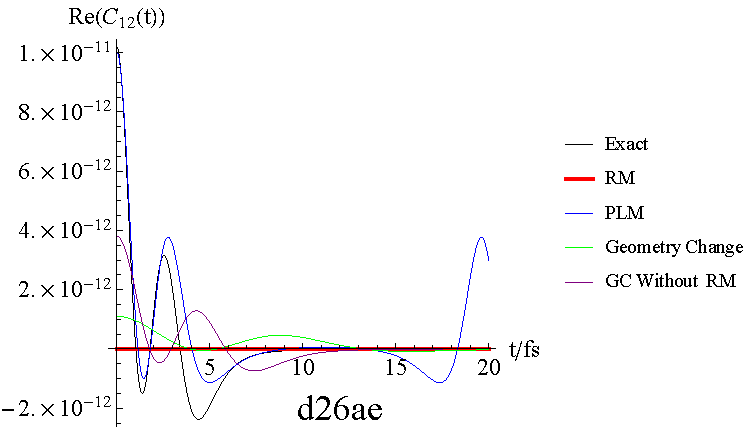
\includegraphics[width=0.78\columnwidth]{Chapters/chap3/Figure10b.pdf}}\\
% \subfloat[]{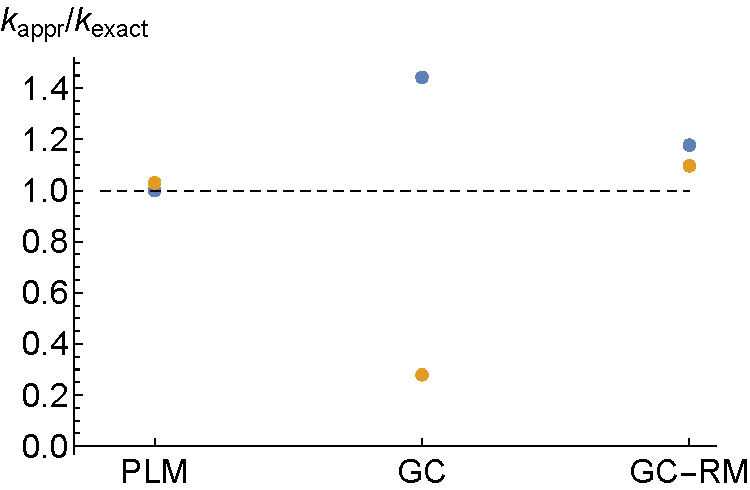
\includegraphics[width=0.53\columnwidth]{Chapters/chap3/Figure10c.pdf}}
\caption{Correlation functions of relaxation mode (RM), PLM, geometry change (GC), and geometry change with the RM component eliminated for (a) c-1,4ee and (b) d-2,6ae. The exact rate is computed using the full set of normal modes.}
\label{Corr}
\end{figure*}

%The procedure is same as before except the relaxation mode is used instead of the PLM.
Since the PLM explains the short-time dynamics and can approximate the local geometry changes within the individual
moieties very well, we anticipate that the PLMs facilitate the energy transfer step. To verify
our prediction, we computed correlation functions of the electron/phonon coupling operators
 (Eq. 4) using different  subsets of nuclear motions  to estimate the couplings:
 PLM,  RM,  geometry change (GC) , and
geometry change with the RM component eliminated (GC-RM).
The latter two correspond to taking the total geometric difference between the initial
and final states of the molecule and  projecting this onto normal modes, and to taking the geometric difference and
subtracting off the relaxation mode.
The various correlation functions and rate
constants are summarized in Fig.~\ref{Corr}.
The exact results are obtained by  using all normal modes and couplings.
The PLM gives nearly perfect agreement to the exact calculation  for both the
time-correlation functions (Fig.~\ref{Corr})  and the computed rates for both molecules considered  (Fig.~\ref{RateComp}.
The relaxation mode (RM) gives no contribution to the correlation function or the rate.
Finally, using just the over-all geometric change (GC) gives a poor estimate of both the correlation
function and the rate.   GC-RM gives the initial transient dynamics in the correlation function and
a reasonable approximation to  the overall rate.  However, the best agreement overall is
obtained by using the PLM identified using the Lanczos search algorithm.



%The results are consistent with our intuition.  The relaxation mode a gives negligible correlation
%function, so its contribution to the rate constant can be neglected.
%Using just the geometry change gives a reasonable rate and it gets even better when the RM component is removed, but
%neither of them beats the PLM.  GC-RM
%%The difference of bond lengths and angles are listed in Table. ~\ref{aprroxGeom}.
%



%Using the relaxation mode rather than the PLM we see that being the
%dominant mode in geometry change, relaxation mode gives much poorer approximation for
%both bond lengths and angles, which is reasonable due to the different nature of the internal and gross motions.
%%It is expected as we understand there are two types of motions here.
%
%


\begin{figure*}[!t]
\subfloat[]{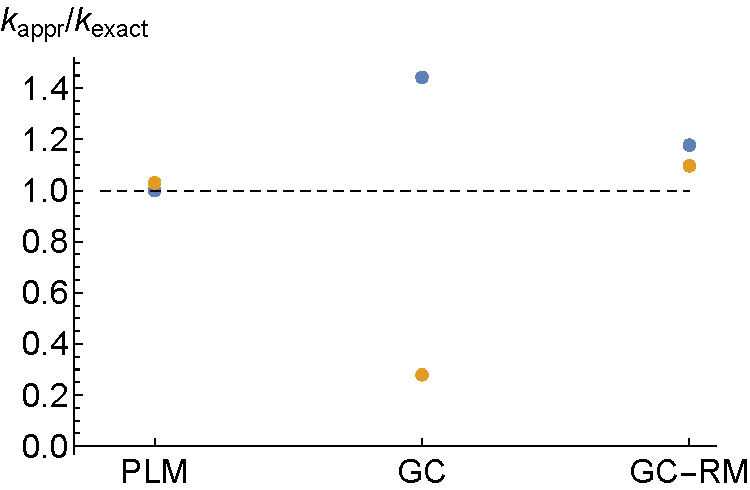
\includegraphics[width=0.9\columnwidth]{Chapters/chap3/Figure10c.pdf}}
\caption{Relative comparison of the rate constants computed using different sets of reduced modes. blue = c-1,4ee, gold =d-2,6ae. }
\label{RateComp}
\end{figure*}




\section{Discussion}
%From the significance of relaxation mode in geometry change and its negligible role in rate
%constant we conclude that the entire transfer process consists of two steps, in the agreement
%of Born-Oppenheimer approximation. At first, the excited electron in donor moiety de-excites
%while one electron in acceptor moiety gets excited. This fast transfer is facilitated by PLM
%and changes bond lengths of donor and acceptor fragments in a totally symmetric way,
%agreeing with the form of HOMO/LUMO. After the exciton transfer, the entire molecule
%undergo es slow but relatively large relaxation under the new electron distribution.  The change
%is mainly the gross motions of fragments so mainly torsional normal modes with very low
%frequencies are involved. This works clarifies the role of shows the primary Lanczos mode.
%It participates the reaction mainly in the short-time fast transfer step, and is the collection
%of normal modes in a way that implicit knowledge of HOMO/LUMO is included.  We also
%show the power of our methodology in analyzing nuclear motions. We are able to discuss
%the contributions of certain directions in rate constants and their roles in transfer.   By
%investigating PLM and geometry change, we detail the picture of transfer in agreement with
%the Born-Oppenheimer approximation. In the future, we can apply our method to study
%dynamics of other systems. We are trying it for molecules involving bond breaking. If
%succeeded, our approach can be useful in the study of selective reaction.


We presented here a further exploration of the classes of nuclear motions that accompany
and electronic energy transition.
% Our approach  is similar to the way Google and Netflix ranks
% page-hits or movie preferences based upon similarity to a set of search criteria identifies
% a subset of nuclear motions that are most strongly coupled to the transition and ranks them according to the
% coupling strength.
We show that deeper insight can be gained by analyzing the primary  modes
and comparing them to both the geometric distortion of the molecule and to the electronic orbitals
involved in the transition.

Our results also suggest that the energy-transfer process in these systems occurs in two distinct steps.
The initial transfer from the donor to acceptor occurs in a fixed nuclear frame--as per the Condon principle.
This fast transfer is facilitated by the PLM and  involves excitations  in the C=C bond lengths of
donor and acceptor fragments in accordance with changes in the HOMO/LUMO populations of each fragment.
 After the exciton transfer, the entire molecule
undergoes a slow but large geometric relaxation under the new electronic distribution.

Finally, we emphasize that the PLM approach and this analysis need not be limited to
the energy transfer cases studied here.  Combined with the time-convolutionless master equation
approach, this provides  a robust and efficient way for computing state-to-state  transitions rates
for a wide class of molecular systems.

% \begin{acknowledgments}
% This work was funded in part by grants from  the National Science
% Foundation (CHE-1362006) and the Robert A. Welch Foundation (E-1337).
% We thank Dr. Hao Li for useful comments and suggestions.
% \end{acknowledgments}

% \bibliography{Dbib}

% \bibliography{fragmentanalysis}
%merlin.mbs aipnum4-1.bst 2010-07-25 4.21a (PWD, AO, DPC) hacked
%Control: key (0)
%Control: author (8) initials jnrlst
%Control: editor formatted (1) identically to author
%Control: production of article title (-1) disabled
%Control: page (0) single
%Control: year (1) truncated
%Control: production of eprint (0) enabled
% \begin{thebibliography}{16}%
% \makeatletter
% \providecommand \@ifxundefined [1]{%
%  \@ifx{#1\undefined}
% }%
% \providecommand \@ifnum [1]{%
%  \ifnum #1\expandafter \@firstoftwo
%  \else \expandafter \@secondoftwo
%  \fi
% }%
% \providecommand \@ifx [1]{%
%  \ifx #1\expandafter \@firstoftwo
%  \else \expandafter \@secondoftwo
%  \fi
% }%
% \providecommand \natexlab [1]{#1}%
% \providecommand \enquote  [1]{``#1''}%
% \providecommand \bibnamefont  [1]{#1}%
% \providecommand \bibfnamefont [1]{#1}%
% \providecommand \citenamefont [1]{#1}%
% \providecommand \href@noop [0]{\@secondoftwo}%
% \providecommand \href [0]{\begingroup \@sanitize@url \@href}%
% \providecommand \@href[1]{\@@startlink{#1}\@@href}%
% \providecommand \@@href[1]{\endgroup#1\@@endlink}%
% \providecommand \@sanitize@url [0]{\catcode `\\12\catcode `\$12\catcode
%   `\&12\catcode `\#12\catcode `\^12\catcode `\_12\catcode `\%12\relax}%
% \providecommand \@@startlink[1]{}%
% \providecommand \@@endlink[0]{}%
% \providecommand \url  [0]{\begingroup\@sanitize@url \@url }%
% \providecommand \@url [1]{\endgroup\@href {#1}{\urlprefix }}%
% \providecommand \urlprefix  [0]{URL }%
% \providecommand \Eprint [0]{\href }%
% \providecommand \doibase [0]{http://dx.doi.org/}%
% \providecommand \selectlanguage [0]{\@gobble}%
% \providecommand \bibinfo  [0]{\@secondoftwo}%
% \providecommand \bibfield  [0]{\@secondoftwo}%
% \providecommand \translation [1]{[#1]}%
% \providecommand \BibitemOpen [0]{}%
% \providecommand \bibitemStop [0]{}%
% \providecommand \bibitemNoStop [0]{.\EOS\space}%
% \providecommand \EOS [0]{\spacefactor3000\relax}%
% \providecommand \BibitemShut  [1]{\csname bibitem#1\endcsname}%
% \let\auto@bib@innerbib\@empty
% %</preamble>
% \bibitem [{\citenamefont {Marcus}(1956)}]{marcus1956theory}%
%   \BibitemOpen
%   \bibfield  {author} {\bibinfo {author} {\bibfnamefont {R.~A.}\ \bibnamefont
%   {Marcus}},\ }\href@noop {} {\bibfield  {journal} {\bibinfo  {journal} {The
%   Journal of Chemical Physics}\ }\textbf {\bibinfo {volume} {24}},\ \bibinfo
%   {pages} {966} (\bibinfo {year} {1956})}\BibitemShut {NoStop}%
% \bibitem [{\citenamefont {Marcus}(1965)}]{marcus1965theory}%
%   \BibitemOpen
%   \bibfield  {author} {\bibinfo {author} {\bibfnamefont {R.~A.}\ \bibnamefont
%   {Marcus}},\ }\href@noop {} {\bibfield  {journal} {\bibinfo  {journal} {The
%   Journal of Chemical Physics}\ }\textbf {\bibinfo {volume} {43}},\ \bibinfo
%   {pages} {679} (\bibinfo {year} {1965})}\BibitemShut {NoStop}%
% \bibitem [{\citenamefont {Marcus}(1993)}]{marcus1993electron}%
%   \BibitemOpen
%   \bibfield  {author} {\bibinfo {author} {\bibfnamefont {R.~A.}\ \bibnamefont
%   {Marcus}},\ }\href@noop {} {\bibfield  {journal} {\bibinfo  {journal}
%   {Reviews of Modern Physics}\ }\textbf {\bibinfo {volume} {65}},\ \bibinfo
%   {pages} {599} (\bibinfo {year} {1993})}\BibitemShut {NoStop}%
% \bibitem [{\citenamefont {Miller}, \citenamefont {Calcaterra},\ and\
%   \citenamefont {Closs}(1984)}]{miller1984intramolecular}%
%   \BibitemOpen
%   \bibfield  {author} {\bibinfo {author} {\bibfnamefont {J.}~\bibnamefont
%   {Miller}}, \bibinfo {author} {\bibfnamefont {L.}~\bibnamefont {Calcaterra}},
%   \ and\ \bibinfo {author} {\bibfnamefont {G.}~\bibnamefont {Closs}},\
%   }\href@noop {} {\bibfield  {journal} {\bibinfo  {journal} {Journal of the
%   American Chemical Society}\ }\textbf {\bibinfo {volume} {106}},\ \bibinfo
%   {pages} {3047} (\bibinfo {year} {1984})}\BibitemShut {NoStop}%
% \bibitem [{\citenamefont {Closs}\ \emph {et~al.}(1988)\citenamefont {Closs},
%   \citenamefont {Piotrowiak}, \citenamefont {MacInnis},\ and\ \citenamefont
%   {Fleming}}]{closs1988determination}%
%   \BibitemOpen
%   \bibfield  {author} {\bibinfo {author} {\bibfnamefont {G.~L.}\ \bibnamefont
%   {Closs}}, \bibinfo {author} {\bibfnamefont {P.}~\bibnamefont {Piotrowiak}},
%   \bibinfo {author} {\bibfnamefont {J.~M.}\ \bibnamefont {MacInnis}}, \ and\
%   \bibinfo {author} {\bibfnamefont {G.~R.}\ \bibnamefont {Fleming}},\
%   }\href@noop {} {\bibfield  {journal} {\bibinfo  {journal} {Journal of the
%   American Chemical Society}\ }\textbf {\bibinfo {volume} {110}},\ \bibinfo
%   {pages} {2652} (\bibinfo {year} {1988})}\BibitemShut {NoStop}%
% \bibitem [{\citenamefont {Closs}\ \emph {et~al.}(1989)\citenamefont {Closs},
%   \citenamefont {Johnson}, \citenamefont {Miller},\ and\ \citenamefont
%   {Piotrowiak}}]{closs1989connection}%
%   \BibitemOpen
%   \bibfield  {author} {\bibinfo {author} {\bibfnamefont {G.~L.}\ \bibnamefont
%   {Closs}}, \bibinfo {author} {\bibfnamefont {M.~D.}\ \bibnamefont {Johnson}},
%   \bibinfo {author} {\bibfnamefont {J.~R.}\ \bibnamefont {Miller}}, \ and\
%   \bibinfo {author} {\bibfnamefont {P.}~\bibnamefont {Piotrowiak}},\
%   }\href@noop {} {\bibfield  {journal} {\bibinfo  {journal} {Journal of the
%   American Chemical Society}\ }\textbf {\bibinfo {volume} {111}},\ \bibinfo
%   {pages} {3751} (\bibinfo {year} {1989})}\BibitemShut {NoStop}%
% \bibitem [{\citenamefont {Pereverzev}\ and\ \citenamefont
%   {Bittner}(2006)}]{pereverzev2006time}%
%   \BibitemOpen
%   \bibfield  {author} {\bibinfo {author} {\bibfnamefont {A.}~\bibnamefont
%   {Pereverzev}}\ and\ \bibinfo {author} {\bibfnamefont {E.~R.}\ \bibnamefont
%   {Bittner}},\ }\href {\doibase 10.1063/1.2348869} {\bibfield  {journal}
%   {\bibinfo  {journal} {The Journal of Chemical Physics}\ }\textbf {\bibinfo
%   {volume} {125}},\ \bibinfo {eid} {104906} (\bibinfo {year}
%   {2006})}\BibitemShut {NoStop}%
% \bibitem [{\citenamefont {Tamura}\ \emph {et~al.}(2008)\citenamefont {Tamura},
%   \citenamefont {Ramon}, \citenamefont {Bittner},\ and\ \citenamefont
%   {Burghardt}}]{tamura2008phonon}%
%   \BibitemOpen
%   \bibfield  {author} {\bibinfo {author} {\bibfnamefont {H.}~\bibnamefont
%   {Tamura}}, \bibinfo {author} {\bibfnamefont {J.~G.~S.}\ \bibnamefont
%   {Ramon}}, \bibinfo {author} {\bibfnamefont {E.~R.}\ \bibnamefont {Bittner}},
%   \ and\ \bibinfo {author} {\bibfnamefont {I.}~\bibnamefont {Burghardt}},\
%   }\href {\doibase 10.1103/PhysRevLett.100.107402} {\bibfield  {journal}
%   {\bibinfo  {journal} {Physical Review Letters}\ }\textbf {\bibinfo {volume}
%   {100}},\ \bibinfo {eid} {107402} (\bibinfo {year} {2008})}\BibitemShut
%   {NoStop}%
% \bibitem [{\citenamefont {Tamura}, \citenamefont {Bittner},\ and\ \citenamefont
%   {Burghardt}(2007)}]{tamura2007exciton}%
%   \BibitemOpen
%   \bibfield  {author} {\bibinfo {author} {\bibfnamefont {H.}~\bibnamefont
%   {Tamura}}, \bibinfo {author} {\bibfnamefont {E.~R.}\ \bibnamefont {Bittner}},
%   \ and\ \bibinfo {author} {\bibfnamefont {I.}~\bibnamefont {Burghardt}},\
%   }\href {\doibase 10.1063/1.2431358} {\bibfield  {journal} {\bibinfo
%   {journal} {The Journal of Chemical Physics}\ }\textbf {\bibinfo {volume}
%   {126}},\ \bibinfo {eid} {021103} (\bibinfo {year} {2007})}\BibitemShut
%   {NoStop}%
% \bibitem [{\citenamefont {Singh}\ \emph {et~al.}(2009)\citenamefont {Singh},
%   \citenamefont {Bittner}, \citenamefont {Beljonne},\ and\ \citenamefont
%   {Scholes}}]{singh2009fluorescence}%
%   \BibitemOpen
%   \bibfield  {author} {\bibinfo {author} {\bibfnamefont {J.}~\bibnamefont
%   {Singh}}, \bibinfo {author} {\bibfnamefont {E.~R.}\ \bibnamefont {Bittner}},
%   \bibinfo {author} {\bibfnamefont {D.}~\bibnamefont {Beljonne}}, \ and\
%   \bibinfo {author} {\bibfnamefont {G.~D.}\ \bibnamefont {Scholes}},\ }\href
%   {\doibase 10.1063/1.3259549} {\bibfield  {journal} {\bibinfo  {journal} {The
%   Journal of Chemical Physics}\ }\textbf {\bibinfo {volume} {131}},\ \bibinfo
%   {eid} {194905} (\bibinfo {year} {2009})}\BibitemShut {NoStop}%
% \bibitem [{\citenamefont {Bittner}\ and\ \citenamefont
%   {Silva}(2014)}]{bittner2014noise}%
%   \BibitemOpen
%   \bibfield  {author} {\bibinfo {author} {\bibfnamefont {E.~R.}\ \bibnamefont
%   {Bittner}}\ and\ \bibinfo {author} {\bibfnamefont {C.}~\bibnamefont
%   {Silva}},\ }\href {http://dx.doi.org/10.1038/ncomms4119} {\bibfield
%   {journal} {\bibinfo  {journal} {Nature Communications}\ }\textbf {\bibinfo {volume}
%   {5}},\ \bibinfo {pages} {3119} (\bibinfo {year} {2014})}\BibitemShut
%   {NoStop}%
% \bibitem [{\citenamefont {Yang}\ and\ \citenamefont
%   {Bittner}(2014)}]{yang2014intramolecular}%
%   \BibitemOpen
%   \bibfield  {author} {\bibinfo {author} {\bibfnamefont {X.}~\bibnamefont
%   {Yang}}\ and\ \bibinfo {author} {\bibfnamefont {E.~R.}\ \bibnamefont
%   {Bittner}},\ }\href@noop {} {\bibfield  {journal} {\bibinfo  {journal} {The
%   Journal of Physical Chemistry A}\ }\textbf {\bibinfo {volume} {118}},\
%   \bibinfo {pages} {5196} (\bibinfo {year} {2014})}\BibitemShut {NoStop}%
% \bibitem [{\citenamefont {Subotnik}\ \emph {et~al.}(2010)\citenamefont
%   {Subotnik}, \citenamefont {Vura-Weis}, \citenamefont {Sodt},\ and\
%   \citenamefont {Ratner}}]{subotnik2010predicting}%
%   \BibitemOpen
%   \bibfield  {author} {\bibinfo {author} {\bibfnamefont {J.~E.}\ \bibnamefont
%   {Subotnik}}, \bibinfo {author} {\bibfnamefont {J.}~\bibnamefont {Vura-Weis}},
%   \bibinfo {author} {\bibfnamefont {A.~J.}\ \bibnamefont {Sodt}}, \ and\
%   \bibinfo {author} {\bibfnamefont {M.~A.}\ \bibnamefont {Ratner}},\
%   }\href@noop {} {\bibfield  {journal} {\bibinfo  {journal} {The Journal of
%   Physical Chemistry A}\ }\textbf {\bibinfo {volume} {114}},\ \bibinfo {pages}
%   {8665} (\bibinfo {year} {2010})}\BibitemShut {NoStop}%
% \bibitem [{\citenamefont {Grover}\ and\ \citenamefont
%   {Silbey}(1970)}]{grover1970exciton}%
%   \BibitemOpen
%   \bibfield  {author} {\bibinfo {author} {\bibfnamefont {M.~K.}\ \bibnamefont
%   {Grover}}\ and\ \bibinfo {author} {\bibfnamefont {R.}~\bibnamefont
%   {Silbey}},\ }\href@noop {} {\bibfield  {journal} {\bibinfo  {journal} {The
%   Journal of Chemical Physics}\ }\textbf {\bibinfo {volume} {52}},\ \bibinfo
%   {pages} {2099} (\bibinfo {year} {1970})}\BibitemShut {NoStop}%
% \bibitem [{\citenamefont {Rice}\ and\ \citenamefont
%   {Gartstein}(1994)}]{rice1994excitons}%
%   \BibitemOpen
%   \bibfield  {author} {\bibinfo {author} {\bibfnamefont {M.}~\bibnamefont
%   {Rice}}\ and\ \bibinfo {author} {\bibfnamefont {Y.~N.}\ \bibnamefont
%   {Gartstein}},\ }\href@noop {} {\bibfield  {journal} {\bibinfo  {journal}
%   {Physical review letters}\ }\textbf {\bibinfo {volume} {73}},\ \bibinfo
%   {pages} {2504} (\bibinfo {year} {1994})}\BibitemShut {NoStop}%
% \bibitem [{\citenamefont {Dexter}(1953)}]{dexter1953theory}%
%   \BibitemOpen
%   \bibfield  {author} {\bibinfo {author} {\bibfnamefont {D.~L.}\ \bibnamefont
%   {Dexter}},\ }\href@noop {} {\bibfield  {journal} {\bibinfo  {journal} {The
%   Journal of Chemical Physics}\ }\textbf {\bibinfo {volume} {21}},\ \bibinfo
%   {pages} {836} (\bibinfo {year} {1953})}\BibitemShut {NoStop}%
% \end{thebibliography}%


% \end{document}
%
% ****** End of file template.aps ******
